% +--------------------------------------------------------------------+
% | The LaTex keyword \documentclass selects a particular class to     |
% | associate with the document.  The current documentclass            |
% | {class_diss} generates a Table of Contents that has leading dots   |
% | only on chapter subheadings.  If you prefer a Table of Contents    |
% | that has leading dots for all entries, replace {class_diss}        |
% | with {Mydiss} in the command below.                                |
% |                                                                    |
% +--------------------------------------------------------------------+

\documentclass[final,12pt,oneside]{class_diss}
\bibliographystyle{unsrtnat}

\usepackage{parskip}
\setlength{\parskip}{\baselineskip}%
\setlength{\parindent}{20pt}%
\usepackage[utf8]{inputenc}
\usepackage[T1]{fontenc}
\usepackage[spanish]{babel}
\addto\captionsspanish{%
	\renewcommand{\contentsname}{Índice General}
	\renewcommand{\listfigurename}{Índice de Figuras}
	\renewcommand{\listtablename}{Índice de Tablas}
	\renewcommand{\bibname}{Referencias}
}

%\usepackage{caption}
\usepackage{subcaption}
\usepackage{array}
%\usepackage{     caption2} % Customize captions a bit more
\usepackage{      amsmath} % American Mathematics Society standards
%\usepackage{      wrapfig} % Wraps text around a figure or table
\usepackage{     graphicx} % Extended graphics package.
%\usepackage{     fancyhdr} % Efficiently handles headers and footers
%\usepackage{       braket} % Bra-Ket notation package
%\usepackage{     mathrsfs} % Specialized Math fonts (Hamiltonian, etc.)
%\usepackage{boxedminipage} % Boxed text can be produced
%\usepackage{     setspace} % Controls line spacing via \begin{space}

\usepackage{amsxtra}
\usepackage{amssymb}
\usepackage{amsthm}
\usepackage{latexsym}

\usepackage[usenames]{color}

\definecolor{  Pink}{rgb}{1.0, 0.5, 0.5}
\definecolor{Maroon}{rgb}{0.8, 0.0, 0.0}

\usepackage[sort&compress]{natbib}
\bibpunct{[}{]}{,}{n}{}{}
\usepackage{hypernat}

% Hyperref settings

\usepackage[pdftex, plainpages=false, pdfpagelabels]{hyperref}

\hypersetup{
    linktocpage=true,
    colorlinks=true,
    citecolor=blue,
    urlcolor=red,
    linkcolor=Maroon,
    citebordercolor={1 0 0},
    urlbordercolor={1 0 0},
    linkbordercolor={.7 .8 .8},
    breaklinks=true,
}

\topmargin      = -0.56in
\textheight     =  8.60in
\textwidth      =  6.46in
\oddsidemargin  =  0.02in

\begin{document}

  \setcounter{page}{-1}

% +--------------------------------------------------------------------+
% | Title Page
% +--------------------------------------------------------------------+

\newpage

% No page number

\thispagestyle{empty}

\begin{center}

   \vspace{1cm}

   {\Large GRAPHIC SHADERS FOR SCIENTIFIC VISUALIZATION}\\

   \vspace{0.5cm}

   \vspace{0.5cm}

   {\large DAVID FERNÁNDEZ ALCOBA}\\

   \vspace{0.5cm}

   DOBLE GRADO EN INGENIERÍA INFORMÁTICA - MATEMÁTICAS\\ 
   FACULTAD DE INFORMÁTICA\\
   UNIVERSIDAD COMPLUTESNE DE MADRID \\

   \vspace{0.65cm}
   \rule{2in}{0.5pt}\\
   \vspace{1.85cm}

  
\includegraphics[height=2.5in]{figures/escudo.jpg}
  
   \vspace{1.5cm}
Trabajo de Fin de Grado en Ingeniería Informática - Matemáticas

   \vspace{0.5cm}

  \today\\
   \vspace{1cm}

\end{center}

{\raggedleft
   \vspace{ 1cm}
Directora:\\
   \vspace{ 0.2cm}
Ana Gil Luezas\\
}

   \pdfbookmark[0]{Portada}{PDFPortadaPage}

%% +--------------------------------------------------------------------+
% | Copyright Page
% +--------------------------------------------------------------------+

\newpage

\thispagestyle{empty}

\begin{center}

{\bf \Huge Autorización de difusión}

\vspace{1cm}

% +--------------------------------------------------------------------+
% | On the line below, replace "Enter Your Name" with your name
% | Use the same form of your name as it appears on your title page.
% | Use mixed case, for example, Lori Goetsch.
% +--------------------------------------------------------------------+

   \large David Fernández Alcoba\\

   \vspace{0.5cm}

% +--------------------------------------------------------------------+
% | On the line below, replace Fecha
% |
% +--------------------------------------------------------------------+

   \today\\

   \vspace{0.5cm}
   \end{center}
   
El/la abajo firmante, matriculado/a en el Doble Grado en Ingeniería Informática y Matemáticas de la Facultad de Informática, autoriza a la Universidad Complutense de Madrid (UCM) a difundir y utilizar con fines académicos, no comerciales y mencionando expresamente a su autor el presente Trabajo Fin de Grado “GRAPHIC SHADERS FOR SCIENTIFIC VISUALIZATION”, realizado durante el curso académico 2018-2019 bajo la dirección de Ana Gil Luezas en el Departamento de Sistemas Informáticos y Computación, y a la Biblioteca de la UCM a depositarlo en el Archivo Institucional E-Prints Complutense con el objeto de incrementar la difusión, uso e impacto del trabajo en Internet y garantizar su preservación y acceso a largo plazo.

	\vspace{2.5cm}
	\raggedleft{David Fernández Alcoba}

%   \pdfbookmark[0]{Autorización}{PDFAutorizacionPage}

% +--------------------------------------------------------------------+ |
% Copyright Page
% +--------------------------------------------------------------------+

\newpage

\thispagestyle{empty}

\begin{center}

{\bf \Huge Resumen en castellano}

  \end{center} \vspace{1cm}

Las GPUs se utilizan normalmente para juegos y aplicaciones gráficas similares,
prestando menos atención a otros aspectos en los que pueden ser útiles, como lo
es la visualización científica. En este trabajo se analiza la utilidad de los
shaders para problemas de este tipo, demostrando la capacidad de cada uno de sus
tipos (vertex, tesselation, geometry, fragment). Además, se introducen ejemplos
de conjuntos de datos y modelos reales para ilustrar su capacidad, concretamente
utilizando técnicas de visualización de imágenes, modelos y renderizado de
superficies. El resultado es una aplicación de visualización científica en la
que el usuario puede cargar sus propios modelos y aplicar sobre ellos algunas de
las técnicas propuestas. Como posible trabajo futuro, se propone la extensión de
la aplicación con otras de las técnicas conocidas de visualización científica.

\vspace{1cm}

% +--------------------------------------------------------------------+ | On
% the line below, replace Fecha |
% +--------------------------------------------------------------------+

\begin{center}

{\bf \Large Palabras clave}

   \end{center}

   \vspace{0.5cm}
   
   Lista de palabras clave
   



   \pdfbookmark[0]{Resumen}{PDFResumenPage}

% +--------------------------------------------------------------------+
% | Copyright Page
% +--------------------------------------------------------------------+

\newpage

\thispagestyle{empty}

\begin{center}

{\bf \Huge Abstract}

  \end{center}
\vspace{1cm}

English version of the abstract

\vspace{1cm}

% +--------------------------------------------------------------------+
% | On the line below, replace Fecha
% |
% +--------------------------------------------------------------------+

\begin{center}

{\bf \Large Keywords}

   \end{center}

   \vspace{0.5cm}
   
List of keywords
   



	\pdfbookmark[0]{Abstract}{PDFAbstractPage}

 \vfill

%\thispagestyle{empty} Looks like it's ok to remove this line
\newpage
\pagenumbering{roman}

\setcounter{page}{4}

\phantomsection

\addcontentsline{toc}{chapter}{Índice General}
\tableofcontents

\addcontentsline{toc}{chapter}{Índice de Figuras}
\listoffigures

\listoftables
\addcontentsline{toc}{chapter}{Índice de Tablas}

\hfill  %Are these lines necessary?
\hfill

\newpage
\pagenumbering{arabic}
\setcounter{page}{1}

\cleardoublepage

\chapter{Introducción}
\label{makereference}

Tal y como se cuenta en~\citet{DEFANTI1991247}, los científicos computacionales
basan su trabajo en fuentes de datos de gran volumen. Sin embargo, estos datos
tienen tal magnitud que los científicos se ven, a menudo, superados. Entre las
fuentes de datos de gran volumen se encuentran:

\begin{itemize}
		\item Supercomputadores
		\item Inteligencia militar, satélites, datos astronómicos y de tiempo atmosférico
		\item Sondas enviando datos desde otros planetas
		\item Radio telescopios terrestres
		\item Instrumentos capturando temperaturas oceánicas, movimientos tectónicos y 
				actividad volcánica y sísmica
		\item Escáneres médicos empleando distintas técnicas de imagen como tomografía, 
				resonancias magnéticas, etc
\end{itemize}

Simplemente con un formato numérico, el cerebro humano es incapaz de interpretar
gigabytes de datos cada día, resultando en mucha información desperdiciada. De
aquí surge la necesidad de una alternativa a los números. La posibilidad de los
científicos para visualizar cómputos complejos y simulaciones es absolutamente
esencial para asegurar la integridad de análisis y predicciones, así como
presentar esta información al resto.

Esta capacidad de visualización se hace especialmente importante en el ser
humano, puesto que, de todas nuestras funciones cerebrales, nuestro sistema de
visión es el que mayor capacidad de procesamiento de información tiene. Según
expertos en conocimiento, el procesamiento de información en humanos tiene dos
formas: preconsciente y consciente. El procesamiento de información
preconsciente es involuntario, similar a la respiración. Este es el tipo de
procesamiento que se da en información gráfica.
~\citet{Rohrer:2000:SBI:510378.510552}

Teniendo esto en cuenta y el hecho de que cada persona tiene una capacidad de
vision espacial diferente, la informática gráfica puede ayudar a aquellos que
tienen una mayor dificultad y que, de otro modo, serían incapaces de visualizar
conceptos complejos.

Estos hechos muestran una necesidad ha resultado en el surgimiento, en la última
década, de una disciplina totalmente independiente, la visualización científica. 

\section{Motivación}
\label{makereference1.1}

La importancia de lo expuesto anteriormente sirve como suficiente motivación,
aunque a esto se ha de añadir el reto personal de, con este trabajo, aprender y
entender un área de la informática que no forma parte del itinerario en mi
formación, como es la informática gráfica, y que engloba muchas de las materias
vistas hasta ahora tanto en ingeniería informática como en matemáticas.

Además, esta rama dentro de la investigación científica es relativamente
reciente, asociándose su nacimiento en 1987 al
artículo~\citet{McCormick:1988:VSC:43965.43966}, por lo que aún hay muchos retos
y problemas por resolver, haciendo su estudio muy interesante.

\section{Objetivos}
\label{makereference1.2}

El objetivo principal de este trabajo es el de aprender el funcionamiento básico
de los gráficos y la aplicación de éstos a la investigación científica.  Este
objetivo se puede desglosar en otros subobjetivos más concretos y que marcan la
línea de trabajo:

\begin{enumerate}
		\item Comprender el pipeline de gráficos y la utilidad y funcionamiento
				de los shaders, así como aprender el lenguaje GLSL para su
				escritura.
		\item Aprender las técnicas más conocidas de visualización científica y
				cómo desarrollar shaders que las implementen.
		\item Desarrollar una aplicación que ponga de manifiesto lo aprendido,
				desarrollando shaders que ilustren algunas de las técnicas
				vistas.
\end{enumerate}

\section{Plan de trabajo}
\label{makereference1.3}

Con estos objetivos en mente, se desarrolló el siguiente plan de trabajo,
acordado en reuniones iniciales entre tutora y autor del trabajo.

\begin{itemize}
		\item \textbf{Toma de contacto con OpenGL} Durante esta fase se leyeron
				tutoriales sobre OpenGL y se experimentó con diversos shaders y
				librerías para familiarizarse con la tecnología, a la vez que se
				aprendía el lenguaje GLSL.
		\item \textbf{Documentación} Durante la duración completa del proyecto
				se llevó a cabo una documentación acerca de las distintas
				fuentes de información, con el objetivo de no olvidar incluir
				partes importantes en la memoria.
		\item \textbf{Comunicación con el tutor} Se concretaron diversas
				reuniones con la tutora durante las partes intensivas del
				proyecto con el fin de mostrar avances y acordar los siguientes
				pasos. Asimismo, se mantuvo una comunicación mediante correo
				electrónico para aquellas dudas menores que surgieron durante la
				realización del trabajo.
		\item \textbf{Preparación del entorno de desarrollo} Durante esta fase
				se preparó el equipo, instalando las librerías y programas
				necesarios para el correcto funcionamiento de la aplicación.
		\item \textbf{Desarrollo de la aplicación} Una vez preparado el entorno,
				se continuó durante toda la duración del trabajo con el
				desarrollo de la aplicación, incluyendo cada vez nuevas
				capacidades.
		\item \textbf{Redacción de la memoria} Se inició la redacción de la
				memoria una vez se tenían conocimientos suficientes, a mitad de
				la elaboración del trabajo. Una vez comenzada la redacción, se
				fue reeditando y mejorando en un proceso iterativo.
\end{itemize}

\section{Estructura de la memoria}
\label{makereference1.4}

El siguiente capítulo, \textbf{OpenGL y DirectX}~\ref{makereference2}, presenta
las dos grandes especificaciones dentro de la informática gráfica, centrándose
en OpenGL y analizando sus características, capacidades y debilidades, así como
las diferencias entre ambas.

Posteriormente, el capítulo \textbf{Shaders y Visualización
Científica}~\ref{makereference3} explora las técnicas más comunes dentro del
campo de visualización científica y qué tipos de shaders son útiles para cada
una de ellas, introduciendo algunos de los que más adelante se presentarán junto
a la aplicación.

En el capítulo \textbf{Aplicación}~\ref{makereference4} se presenta la
aplicación desarrollada, explicando el diseño, capacidades, experimentos
realizados\ldots

Por último el capítulo \textbf{Conclusiones y Trabajo
Futuro}~\ref{makereference5} incluye un análisis del trabajo realizado, el nivel
de cumplimiento de los objetivos propuestos y posibles líneas de trabajo
futuro.

\begin{table}[b]
	% \begin{center}
		\begin{tabular}[b]{|c|}
			\hline
			\\
			El código de la aplicación desarrollada puede encontrarse en el
			siguiente enlace:\\
			http://github.com/davidfdezalcoba/TFG\\
			\\
			\hline
		\end{tabular}
	% \end{center}
\end{table}

% +--------------------------------------------------------------------+
% | Sample Chapter 2
% +--------------------------------------------------------------------+

\cleardoublepage

% +--------------------------------------------------------------------+
% | Replace "This is Chapter 2" below with the title of your chapter.
% | LaTeX will automatically number the chapters.
% +--------------------------------------------------------------------+

\chapter{OpenGL y Direct3D}
\label{makereference2}

El objetivo de este capítulo es explicar en qué consiste OpenGL, así como su
pipeline de gráficos, los tipos de shaders que incluye y las diferencias que
presenta con Direct3D, su principal competidor.

\section{¿Qué es?}
\label{makereference2.1}

OpenGL~\cite{OpenGL} se define como una API \textit{(application programming interface)}, que
es simplemente una librería de software para acceder a capacidades del hardware
de gráficos (ver \citet{Shreiner:2009:OPG:1696492}).

OpenGL está diseñado como una interfaz independiente del hardware que puede ser
implementada en muchos sistemas hardware de gráficos diferentes, o completamente
como software, en el caso de que el sistema no posea hardware de gráficos.
OpenGL no proporciona ninguna funcionalidad para describir modelos en tres
dimensiones ni operaciones para leer ficheros (como imágenes JPEG, por ejemplo).
En su lugar, se deben construir los objetos tridimensionales a partir de un
pequeño conjunto de primitivas geométricas---puntos, líneas, triángulos y
parches.---(Ver Sección~\ref{makereference2.3}).

\section{Breve historia de OpenGL}
\label{makereference2.2}

OpenGL nace a principios de los años 90, desarrollada por Silicon Graphics~(SGI).  En
los años 80, Silicon Graphics poseía una API privada denominada IRIS GL,
utilizada para producir gráficos en sus estaciones de trabajo IRIS.
Posteriormente, debido a la pérdida de cuota de mercado, decidió hacer su API
pública. Sin embargo, a causa de problemas con patentes y el hecho de tener
características poco relevantes para los gráficos 3D como la funcionalidad de
ventanas, se decidió reescribir algunas de las partes y se lanzó lo que ahora se
conoce como OpenGL.

Esta nueva especificación consiguió logros importantes para la informática gráfica,
como estandarizar el acceso al hardware gráfico, trasladar a los fabricantes la
responsabilidad del desarrollo de las interfaces con el hardware y delegar la
funcionalidad de ventanas al sistema operativo. Todo esto supuso un gran impacto
en la industria, al ofrecer a los desarrolladores una plataforma de alto nivel
sobre la que trabajar.

En 1992, Silicon Graphics lideró la creación del OpenGL Architecture Review
Board (OpenGL ARB)~\cite{OpenGLARB}, un grupo de empresas del sector que sería
la encargada de mantener y extender la especificación en los años siguientes. El
OpenGL ARB estaba formado por 3Dlabs, Apple, ATI, Dell, IBM, Intel, Nvidia, SGI
and Sun Microsystems.

En el año 2000 surge el grupo Khronos~\cite{Khronos}, una organización sin ánimo
de lucro centrada en la creación de estándares abiertos para permitir la
creación, reproducción multimedia y computación paralela en un amplio abanico de
plataformas y dispositivos.

En otoño de 2006, el OpenGL ARB y los directores de Khronos Group
votaron para transferir el control de OpenGL a Khronos Group. El secretario de
la ARB Jon Leech observó: \textit{``Hemos decidido mover OpenGL a Khronos para
		asegurar la salud futura de OpenGL en todas sus
formas.''}~\cite{OpenGLARB}

Khronos Group anunció en 2015 el lanzamiento de una nueva API llamada
Vulkan~\cite{Vulkan}, llamada a ser la sucesora de OpenGL. De hecho, en un
principio esta API fue bautizada por Khronos como ``La iniciativa OpenGL de
nueva generación''. Se trata de una API similar a OpenGL pero de más bajo nivel,
basada en Mantle, cedida a Khronos por AMD~\cite{AMD}.

La principal característica de Vulkan frente a OpenGL es la posibilidad de
aprovechar los núcleos presentes en la CPU con el fin de incrementar
drásticamente el rendimiento gráfico, además de permitir un mayor control sobre
la GPU, disminuyendo la carga de la CPU.

Junto con Vulkan surgió SPIR-V \textit{(Standard Portable Intermediate
Representation)}~\cite{SPIR}, un lenguaje intermedio de computación paralela y
gráficos, también perteneciente al grupo Khronos. Su principal finalidad era la
permitir a los desarrolladores la creación y distribución de binarios
independientes del dispositivo.

Con su aparición, se pasó de utilizar un compilador de GLSL implementado en cada
controlador de OpenGL a la utilización de shaders ya traducidos a un formato
binario por SPIR-V en Vulkan, mejorando considerablemente la velocidad de
inicialización de la aplicación y el número de shaders a utilizar por escena.

En la actualidad conviven ambas APIs, aconsejándose en algunos casos más
simples la utilización de OpenGL en lugar de Vulkan debido a su mayor facilidad
de uso y menor carga de mantenimiento.

\section{Diseño de OpenGL}
\label{makereference2.3}

OpenGL implementa el llamado pipeline de gráficos o pipeline de renderizado.
Este pipeline consiste en una secuencia de etapas de procesamiento para
convertir datos de una aplicación en una imagen final renderizada. 

\begin{figure}[h]
		\centering
		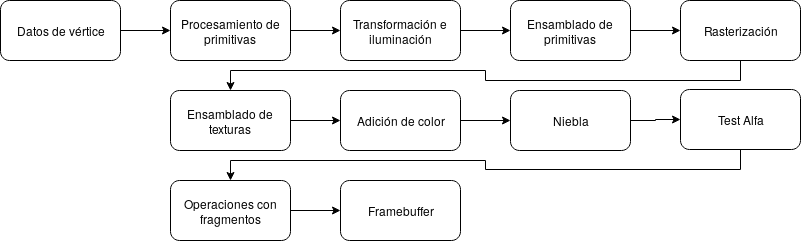
\includegraphics[height=7cm,width=\textwidth]{figures/pipelinefijo.png}
		\caption{Pipeline no programable. OpenGL 1.5}
		\label{fig2.1}
\end{figure}

En un principio, este pipeline de renderizado consistía en varias etapas fijas y
no programables, en las que el programador simplemente elegía una serie de
configuraciones para que OpenGL realizase las operaciones propias de cada etapa.
Las etapas principales de este pipeline eran las siguientes (Ver
Figura~\ref{fig2.1}):

\begin{itemize}
		\item Procesamiento de primitivas
		\item Transformación e iluminación
		\item Ensamblado de primitivas
		\item Rasterización
		\item Ensamblado de texturas
		\item Adición de color
		\item Niebla
		\item Test Alfa
		\item Operaciones con fragmentos
\end{itemize}

Sin embargo, con la versión 2.0 de OpenGL se introdujeron los \textit{shaders},
explorados en detalle en el Capítulo~\ref{makereference3}, que sustituyeron
algunas de estas etapas fijas por etapas programables, dando mayor flexibilidad
al programador. La Figura~\ref{fig2.2} muestra el pipeline asociado a la versión
4.3 de OpenGL. 

\begin{figure}[h]%t=top, b=bottom, h=here
	\begin{subfigure}[b]{.5\textwidth}
		\centering
		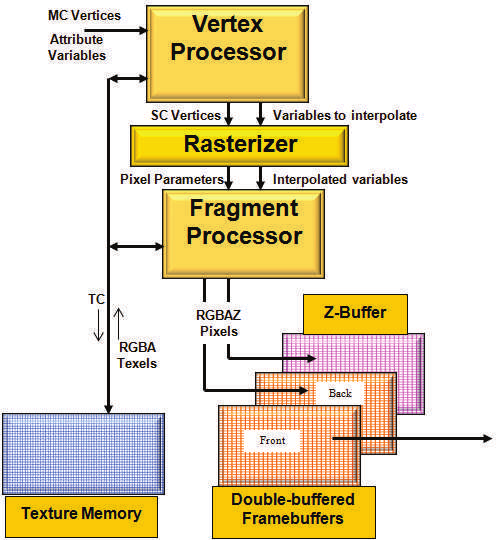
\includegraphics[height=8cm]{figures/pipeline.png}
		\caption{Pipeline de OpenGL}
		\label{fig2.2a}
	\end{subfigure}
	\begin{subfigure}[b]{.5\textwidth}
		\centering
		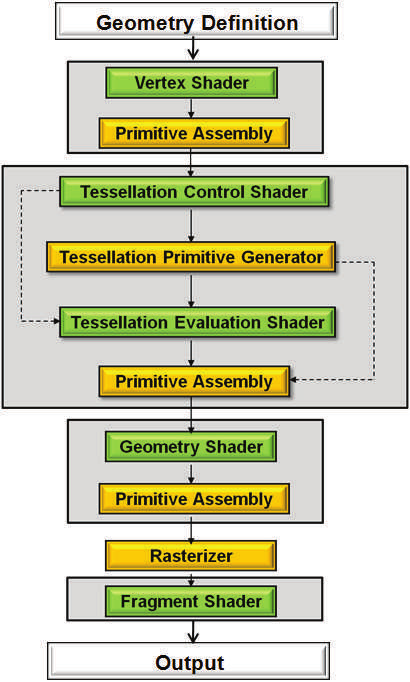
\includegraphics[height=8cm]{figures/pipelineExtendido.png}
		\caption{Pipeline detallado}
		\label{fig2.2b}
	\end{subfigure}
	\caption[Pipeline de gráficos de OpenGL]
	{Pipeline de gráficos de OpenGL. Fuente:~\cite{Bailey}}
	\label{fig2.2}
\end{figure}

El renderizado de una imagen comienza con una llamada, desde la aplicación
principal, a una función de dibujado de OpenGL. Con esta llamada, OpenGL toma
datos sobre vértices contenidos en diferentes objetos y renderiza con estos
datos una o más \textit{primitivas}~\cite{Primitivas}. 

Las primitivas geométricas son las interpretaciones que OpenGL puede
hacer sobre lo que representa un flujo de vértices. Por ejemplo, tres vértices
pueden significar tres puntos independientes, dos líneas, un triángulo, etc.
OpenGL contiene los siguientes tipos principales de primitivas:

\subsection{Primitivas de OpenGL}
\label{ref:primitives}


\subsubsection{Primitivas de Puntos}
\label{ref:points}

OpenGL contiene una única primitiva de puntos: \verb|GL_POINTS|. Cuando se llama
a una función de dibujado con esta primitiva, OpenGL interpreta el flujo de
vértices como puntos independientes.

\subsubsection{Primitivas de Línea}
\label{ref:lines}

En cuanto a las primitivas de línea, hay tres tipos, basándose en distintas
interpretaciones del flujo de vértices.

\begin{itemize}
		\item \verb|GL_LINES|: Los dos primeros vértices se consideran una línea,
				los dos siguientes otra línea, etc.
		\item \verb|GL_LINE_STRIP|: Los vértices adyacentes se consideran una
			línea. Es decir el primero y el segundo forman una línea, el segundo
			y el tercero forman otra línea, etc.
		\item \verb|GL_LINE_LOOP|: Como \verb|GL_LINE_STRIP|, pero el primer y
				último vértices se consideran también una línea.
\end{itemize}

\subsubsection{Primitivas de Triángulo}
\label{ref:triangles}

Un triángulo es una primitiva formada por tres vértices. También existen tres
primitivas de triángulo:

\begin{itemize}
		\item \verb|GL_TRIANGLES|: los tres primeros vértices forman un
				triángulo, los tres siguientes otro, etc.
		\item \verb|GL_TRIANGLE_STRIP|: cada grupo de tres vértices adyacentes
				forman un triángulo. El (0, 1, 2), el (1, 2, 3), etc.
		\item \verb|GL_TRIANGLE_FAN|: El primer vértice queda fijo, y cada grupo
				de dos vértices adyacentes a partir de él forma un triángulo con
				el primero. Por ejemplo el (0, 1, 2), (0, 2, 3), etc.
\end{itemize}

En la Figura~\ref{fig:primitives} se pueden ver las diferentes interpretaciones
en forma de primitiva que puede realizar OpenGL para renderizar un flujo de
vértices. 

\begin{figure}[h]
	\centering	
	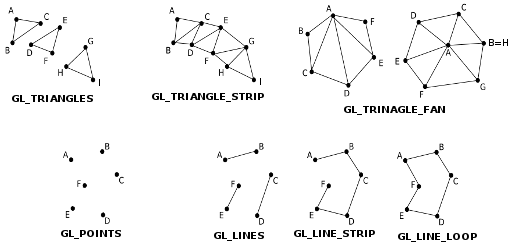
\includegraphics[width=\textwidth]{figures/primitives.png}
	\caption[Primitivas de OpenGL]{Primitivas de OpenGL.
	Fuente:~\cite{PrimitiveImage}}
	\label{fig:primitives}
\end{figure}

Una vez se ha hecho la llamada a la función de dibujado, comienza el proceso de
renderizado, recorriéndose las diferentes etapas que forman el pipeline de
renderizado. 

\subsection{Procesamiento de Vértices}
\label{ref:procesamiento}

La primera etapa del pipeline programable ---Vertex Processor,
Figura~\ref{fig2.2a}---, está formada a su vez por los shaders programables de
vértice, teselación y geométrico \textit{(vertex, tessellation y geometry
shaders)}, que sustituyen a las etapas de transformación e iluminación del
pipeline no programable, así como la etapa fija realizada por OpenGL conocida
como Ensamblado de Primitivas. Obtiene como entrada el flujo de vértices,
normales, definiciones de primitivas geométricas, colores, parámetros de
iluminación, materiales y coordenadas para las texturas. Esta etapa opera sobre
estos datos y los organiza en las primitivas geométricas asociadas en
preparación para la etapa de post-procesado de vértices, en la que se realizan,
entre otras cosas, su recorte y rasterización.  Así, la salida es un conjunto de
vértices como píxeles, con su color, profundidad y coordenadas de textura.

\subsection{Clipping}
\label{ref:clipping}

Posteriormente se realiza el recorte o \textit{clipping}, que ocurre cuando,
ocasionalmente, algunos vértices quedan fuera de lo que se denomina
\textit{viewport}---la región de la ventana donde se permite dibujar---
modificando las primitivas geométricas para que nada quede fuera de ese espacio.
(Ver Figura~\ref{fig2.3a}).

\begin{figure}[h]
	\centering
	\begin{minipage}[b]{0.5\textwidth}
		\centering 
		\captionsetup{justification=centering}
		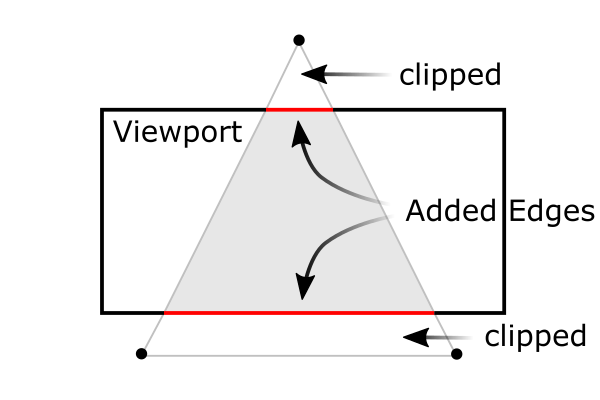
\includegraphics{figures/clipping.png}
		\caption[Clipping en OpenGL.]{Clipping en OpenGL. \\
		Fuente:~\cite{ClippingImage}}
		\label{fig2.3a}
	\end{minipage}\hfill
	\begin{minipage}[b]{0.5\textwidth}
		\centering 
		\captionsetup{justification=centering}
		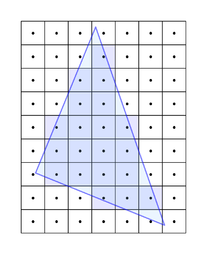
\includegraphics{figures/rasterization.png}
		\caption[Rasterización en OpenGL.]{Rasterización en OpenGL. \\
		Fuente:~\cite{RasterizationImage}}
		\label{fig2.3b}
	\end{minipage}
\end{figure}

\subsection{Rasterización}
\label{ref:rasterizacion}

La siguiente etapa es la rasterización (ver Figura~\ref{fig2.3b}). Este paso
implementa la transición de vértice a fragmento. Inmediatamente después del
clipping, las primitivas geométricas actualizadas se mandan al rasterizador para
la generación de fragmentos. Podemos considerar un fragmento como un ``candidato
a pixel'', en el sentido de que un pixel reside en el \textit{framebuffer}--- un
espacio de memoria manejado por el hardware gráfico que manda al dispositivo de
salida digital--- mientras que un fragmento puede ser rechazado y nunca
actualizar su localización de pixel asociada. 

\subsection{Procesamiento de Fragmentos}
\label{ref:procesamientofrags}

En la última etapa, el procesado de fragmentos se realiza a su vez en dos pasos,
uno de ellos programable con el shader de fragmentos y otro que consta de
distintas operaciones sobre fragmentos realizadas automáticamente por OpenGL.
Durante este último procesamiento, la visibilidad de cada fragmento es
determinada utilizando diferentes tests (profundidad, color, plantilla,
ruido\ldots). 

Cuando un fragmento pasa por todas estas etapas y todos los test activos, puede
ser escrito directamente en el framebuffer, actualizando su color y valor de
profundidad de su pixel o, si el \textit{blending} está activado, mezclando su
color con el del pixel actual para generar un nuevo color que se escribe en el
buffer de fragmentos.

\section{Diferencias con Direct3D}
\label{makereference2.4}

Direct3D es parte del conjunto de la API multimedia DirectX, propiedad de
Microsoft~\cite{Microsoft}. Es la principal competidora de OpenGL, ofreciendo
ambas un conjunto similar de funcionalidades. Aun así, se pueden observar varias
diferencias en términos de disponibilidad, portabilidad, facilidad de uso,
rendimiento, estructura y usuarios finales. En la tabla~\ref{tabla2.1}, se
muestran algunas de ellas resumidas.

\begin{table}[h]
	\centering
	\begin{tabular}{ | m{4cm} | m{5cm} | m{5cm} | }
		\hline
		& OpenGL & Direct3D \\
		\hline
		Soporte de escritorio & Multiplataforma & Microsoft Windows Xbox
		\\
		\hline
		Soporte sistemas empotrados & Multiplataforma (OpenGL ES) & Windows
		Embedded Windows CE \\
		\hline
		Licencia & Libre (con características patentadas) & Privativa
		\\
		\hline
		Usuario final & Profesionales & Juegos \\ 
		\hline
		Lenguaje de shaders & GLSL & HLSL \\
		\hline
	\end{tabular}
	\caption{Diferencias entre OpenGL y Direct3D}
	\label{tabla2.1}
\end{table}

En cuanto a la portabilidad, DirectX solo está disponible para la familia de
sistemas operativos Microsoft Windows, mientras que OpenGL tiene
implementaciones en muchas plataformas, incluyendo Microsoft Windows y sistemas
Unix.

En términos de facilidad de uso hoy en día ambas APIs se encuentran bastante
parejas, habiendo evolucionado desde las primeras versiones, en las que los
desarrolladores instaban a Microsoft a unirse a la iniciativa OpenGL, debido a
que suponía menos esfuerzo trabajar con esta última.

\begin{figure}
	\centering
	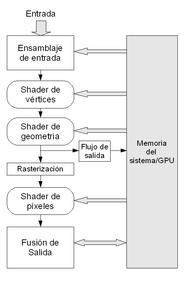
\includegraphics[height=10cm]{figures/directxpipeline.png}
	\caption[Pipeline de gráficos de Direct3D.]{Pipeline de gráficos de
	Direct3D. Fuente:~\cite{3dpipelineimage}}
	\label{fig:differences}
\end{figure}

El diseño de ambas es también similar. Tras muchos años de evolución, el
pipeline gráfico es bastante parecido, como puede apreciarse en la
Figura~\ref{fig:differences}.

Además, las etapas programables del pipeline de OpenGL (vertex, tessellation,
geometry y fragment shader) se escriben en GLSL \textit{OpenGL Shading
Language}~\cite{GLSL}, un lenguaje creado específicamente para este propósito
por el OpenGL ARB. En contraposición, las etapas programables del pipeline
implementado por Direct3D (vertex, geometry y pixel shaders) se escriben en el
lenguaje HLSL \textit{(High Level Shader Language)}~\cite{HLSL} desarrollado por
Microsoft y análogo a GLSL.

En conclusión, hoy en día ambas se consideran bastante similares en cuanto a
rendimiento y capacidades, siendo el soporte a otros sistemas y el carácter de
las licencias las únicas grandes diferencias que hacen decantarse a los
desarrolladores por una u otra.

% +--------------------------------------------------------------------+
% | Sample Chapter 3
% +--------------------------------------------------------------------+

\cleardoublepage

% +--------------------------------------------------------------------+
% | Replace "This is Chapter 3" below with the title of your chapter.
% | LaTeX will automatically number the chapters.
% +--------------------------------------------------------------------+

\chapter{Shaders y Visulización Científica}
\label{makereference3}

Como se ha visto en la sección~\ref{makereference2.3}, el pipeline de gráficos de
OpenGL tiene cuatro etapas programables:

\begin{itemize}
		\item Shader de Vértices (Vertex Shader)
		\item Shaders de Teselación
				\subitem Shader de Control de Teselación (Tessellation Control
				Shader)
				\subitem Shader de Evaluación de Teselación (Tessellation
				Evaluation Shader)
		\item Shader Geométrico (Geometry Shader)
		\item Shader de Fragmento (Fragment Shader)
\end{itemize}

En este capítulo se explicará cómo funcionan, cómo desarrollarlos y cómo
utilizarlos para resolver problemas de visualización científica habituales.

\section{Shaders}
\label{makereference3.1}

Los shaders gráficos son un tipo de programa utilizado inicialmente para
producir niveles apropiados de luz, oscuridad y color en una imagen. Sin
embargo, hoy en día se utilizan con diversas finalidades diferentes como efectos
especiales, post procesado de vídeos, videojuegos, etc.\\

Los shaders se introdujeron en OpenGL en la versión 2.0, incluyendo el lenguaje
de programación centrado en shaders OpenGL Shading Language, también conocido
como GLSL~\cite{GLSL}--- un lenguaje tipo C creado específicamente para que los
desarrolladores tuviesen más control sobre el pipeline de renderizado.---\\

Durante el proceso de desarrollo de shaders no es necesario incluir todas las
etapas que se muestran en la Figura~\ref{fig2.2b}, aunque normalmente, si se
decide utilizar alguno de ellos, se requiere utilizar, al menos, un Vertex
Shader. 

Los shaders del pipeline se comunican entre ellos mediante variables
proporcionadas por GLSL, siendo la salida de un shader la entrada del siguiente,
como se muestra en la Figura~\ref{fig3.1}. Un breve resumen acerca del lenguaje
GLSL se incluye en el Apéndice~\ref{ApendiceA}.

\begin{figure}
		\centering
		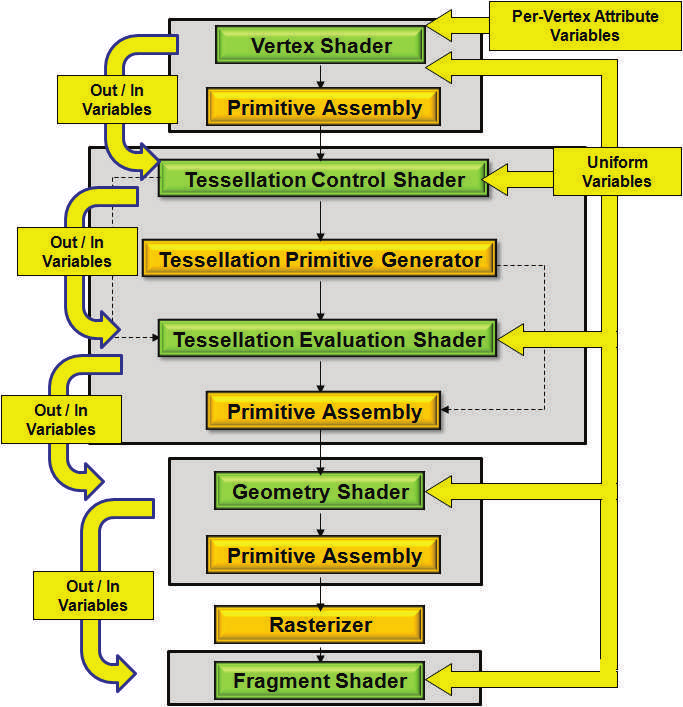
\includegraphics[height=10cm]{figures/variablespipe.png}
		\caption{Comunicación entre shaders del pipeline}
		\label{fig3.1}
\end{figure}

\subsection{Vertex Shader}
\label{ref:Vertex}

El Vertex Shader es la etapa de sombreado en el pipeline de renderizado que se
encarga del procesamiento de los vértices individuales~\cite{VertexShader}. El
Vertex Shader tiene como entrada unos atributos de vértice especificados desde
un \textit{Vertex Array Object (VAO)} por un comando de dibujo. Recibe un único
vértice, formado por sus atributos, del flujo de vértices y genera un único
vértice al flujo de salida. Por cada vértice de entrada ha de haber,
necesariamente, uno de salida. \\

Este shader se invoca una vez por cada vértice en el flujo de entrada,
exceptuando el caso en el que OpenGL detecte que una invocación a este shader
con las exactamente las mismas entradas ya ha sido realizada, en cuyo caso se
reutilizan los resultados de la invocación previa, resultando en un ahorro
de tiempo valioso. \\

Normalmente, las operaciones que se realizan en el Vertex Shader son
transformaciones para el espacio de post-proyección, iluminación por vértice o
preparación para las siguientes etapas del pipeline. \\

\subsection{Tessellation Shaders}
\label{ref:TesShaders}

La Teselación es la etapa, opcional, del pipeline de renderizado que consiste en
subdividir un parche de algún tipo y computar los valores de los nuevos vértices
creados en el proceso. Está compuesta, a su vez, por otras tres etapas, dos de
ellas programables en forma de shader, y una intermedia fija. Cada una de estas
etapas se encarga de una parte del proceso de teselación.\\ 

En esta sección se explican los dos shaders involucrados, además de la etapa
intermedia, llamada generador de primitivas de teselación, pues resulta
importante para entender el proceso y las entradas y salidas a los shaders.

\subsubsection{Tessellation Control Shader}
\label{ref:TesConShader}

El Tessellation Control Shader (TCS)~\cite{TesConShader} es la primera etapa del
proceso de teselación, en el caso de ser utilizado. Se sitúa inmediatamente
posterior al Vertex Shader e inmediatamente anterior al generador de primitivas
de teselación. Controla cuánta teselación provocar en un parche determinado, así
como el tamaño del parche, permitiendo aumentar la cantidad de datos. Su función
principal es la de comunicar al generador de primitivas de teselación el nivel
de teselación deseado, así como proveerle los datos del parche al Tessellation
Evaluation Shader mediante sus variables de salida. \\

Como entrada, el TCS obtiene la salida del Vertex Shader organizada en un vector
de tantos vértices como tenga el parche de entrada. Cada invocación al TCS
produce un único vértice como salida al parche de salida. Por cada vértice en
el parche de entrada se realiza una invocación al TCS, resultando en tantas
invocaciones como vértices hay en dicho parche. \\

En el caso de no utilizar un TCS, se pueden pasar valores por defecto a las
siguientes etapas de teselación.

\subsubsection{Generador de primitivas de teselación}
\label{ref:TesPriGen}

El generador de primitivas de teselación~\cite{TesPriGen} es la etapa que se
encuentra entre los dos shaders de teselación, el TCS y el Tessellation
Evaluation Shader. Esta etapa, fija en el pipeline, es la encargada de crear
nuevas primitivas a partir del parche de entrada. La función principal de este
sistema es la de determinar cuántos vértices crear, en qué orden hacerlo y qué
clase de primitivas construir con ellos. Los datos reales de estos vértices,
como color, posición, etc., han de ser generados por el TES. Debido a esto, el
generador no tiene en cuenta el parche de salida producido por el TCS, sino que
solo opera en términos de teselar un cuadrado o triángulo abstracto, o un bloque
de isolíneas.\\

Esta etapa, está supeditada al Tessellation Evaluation Shader, puesto que solo
se ejecutará en el caso de que exista uno activo. La generación de primitivas en
esta etapa se ve afectada por distintos factores:

\begin{itemize}
		\item Niveles de teselación marcados por el TCS (O por defecto si no hay
				TCS)
		\item Espaciado de los vértices teselados, definido en el TES
		\item Tipo de primitiva, definido en el TES
		\item Orden de generación de primitivas, definido en el TES
\end{itemize}

La cantidad de teselación a realizar se define en niveles de teselación internos
y externos. Funcionan de la siguiente manera: un nivel de teselación 4 indica
que un borde se convertirá en 4 bordes (2 vértices se convertirán en 5). El
nivel externo define el grado de teselación para los bordes externos de la
primitiva. Esto permite que dos parches distintos se conecten apropiadamente, a
pesar de tener distintos niveles de teselación dentro del parche. El nivel
interno hace referencia el número de teselaciones a realizar dentro del parche
abstracto. \\

Cabe destacar que no todos los parches abstractos utilizan los mismos niveles de
teselación. Por ejemplo, los triángulos utilizan un único nivel interno y tres
niveles externos. El resto de posibles niveles son ignorados. \\

El espaciado entre vértices puede realizarse de las siguientes maneras:
espaciado equidistante, espaciado fraccional par o espaciado fraccional impar.

\begin{figure}[h]
	\centering
	\begin{subfigure}{.45\textwidth}
			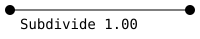
\includegraphics[width=\textwidth]{figures/equal1.png}	
	\end{subfigure}	
	\hfill
	\begin{subfigure}{.45\textwidth}
			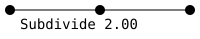
\includegraphics[width=\textwidth]{figures/equal2.png}	
	\end{subfigure}	
	\newline
	\begin{subfigure}{.45\textwidth}
			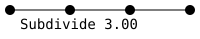
\includegraphics[width=\textwidth]{figures/equal3.png}	
	\end{subfigure}	
	\hfill
	\begin{subfigure}{.45\textwidth}
			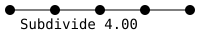
\includegraphics[width=\textwidth]{figures/equal4.png}	
	\end{subfigure}	
	\caption{Teselación - Espaciado equidistante}
	\label{fig3.2}
\end{figure}

El espaciado equidistante (ver Figura~\ref{fig3.2}) divide el borde a teselar
en segmentos de igual longitud. Solo acepta valores enteros, por lo que redondea
el nivel de teselación hasta el siguiente entero. Este hecho causa que los
segmentos aparezcan instantáneamente de un nivel a otro.\\

Para conseguir un comportamiento mas ``suave'' se tienen los otros dos modos de
espaciado. Estos últimos son útiles especialmente cuando el nivel de teselación
es dependiente del área vista desde la cámara. En el espaciado fraccional par el
número de segmentos en los que dividir el borde (nivel de teselación efectivo)
se redondea al siguiente entero par, mientras que en el espaciado fraccional
impar se redondea al siguiente entero impar. Para estos modos de espaciado se
necesita definir dos valores:

\begin{itemize}
		\item $n$, el nivel de teselación efectivo, redondeado según lo
				anterior.
		\item $f$, el valor computado antes del redondeo. Un valor
				potencialmente fraccionario.
\end{itemize}

\begin{figure}
	\centering
	\begin{subfigure}{.45\textwidth}
			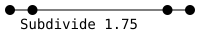
\includegraphics[width=\textwidth]{figures/even1.png}	
	\end{subfigure}
	\hfill
	\begin{subfigure}{.45\textwidth}
			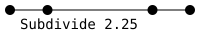
\includegraphics[width=\textwidth]{figures/even2.png}	
	\end{subfigure}
	\newline
	\begin{subfigure}{.45\textwidth}
			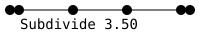
\includegraphics[width=\textwidth]{figures/even3.png}	
	\end{subfigure}
	\hfill
	\begin{subfigure}{.45\textwidth}
			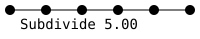
\includegraphics[width=\textwidth]{figures/even4.png}	
	\end{subfigure}
	\caption{Teselación - Espaciado fraccional par}
	\label{fig3.3}
\end{figure}

\begin{figure}
	\centering
	\begin{subfigure}{.45\textwidth}
			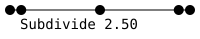
\includegraphics[width=\textwidth]{figures/odd1.png}	
	\end{subfigure}
	\hfill
	\begin{subfigure}{.45\textwidth}
			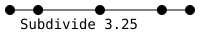
\includegraphics[width=\textwidth]{figures/odd2.png}	
	\end{subfigure}
	\newline
	\begin{subfigure}{.45\textwidth}
			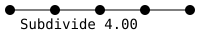
\includegraphics[width=\textwidth]{figures/odd3.png}	
	\end{subfigure}
	\hfill
	\begin{subfigure}{.45\textwidth}
			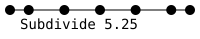
\includegraphics[width=\textwidth]{figures/odd4.png}	
	\end{subfigure}
	\caption{Teselación - Espaciado fraccional impar}
	\label{fig3.4}
\end{figure}

Según este esquema, los bordes a teselar se subdividen en dos conjuntos de
segmentos. El primero con $n-2$ segmentos de igual longitud, el otro con $2$
segmentos de igual longitud entre ellos, pero no necesariamente de igual
longitud que los del el otro conjunto. Estos dos segmentos tendrán menor
longitud que los otros en general. La longitud de estos es exactamente $n-f$.
Por tanto, cuando se cumple que $n-f=0$ se tiene que todos los segmentos tienen
igual longitud. Estos comportamientos se pueden observar en las
Figuras~\ref{fig3.3},~\ref{fig3.4}.

\subsubsection{Tessellation Evaluation Shader}
\label{ref:TesEvaShader}

El Tessellation Evaluation Shader (TES)~\cite{TesEvaShader} es la etapa opcional
que se encuentra entre el generador de primitivas de teselación y el geometry
shader. Su función es la de coger los resultados obtenidos en la etapa anterior
y computar las posiciones interpoladas y otros datos vértice a vértice a partir
de ellos.\\

El TES obtiene del generador de primitivas de teselación un parche abstracto,
así como datos de los vértices para todo el parche, junto con otros datos,
provenientes del TCS. Cada invocación a este shader produce un vértice
particular y es invocado una vez por cada vértice en el parche abstracto.\\

Esta es la etapa donde el programador implementa el algoritmo que se usa para
computar las nuevas posiciones, normales, coordenadas de texturas, etc. Como se
ha expuesto antes, este shader es el que determina si ocurrirá o no la etapa de
generación de primitivas de teselación, puesto que solo se ejecutará si existe
un TES activo.\\

El TES, en caso de ser utilizado, debe especificar el tipo de primitiva que
servirá como entrada al geometry shader. Este tipo puede ser puntos, isolíneas,
triángulos o cuadriláteros.

\subsection{Geometry Shader}
\label{ref:GeoShader}

El Geometry Shader~\cite{GeoShader} es un programa escrito en GLSL que
corresponde a la etapa del pipeline programable que se encuentra entre el TES o
el Vertex Shader (dependiendo de si existe o no teselación) y la etapa fija de
post-procesado de vértices. Este shader es opcional y no es necesaria su
utilización.\\

Las invocaciones a este shader toman como entrada una única primitiva geométrica
y puede dar como salida cero o más primitivas, aunque existe un límite de
primitivas que se pueden generar en cada invocación, dependiendo de la
implementación. Los shaders geométricos están diseñados para aceptar como
entrada una primitiva específica y dar como salida otra. \\

Sus usos varían bastante, pudiéndose utilizar como una manera de amplificar la
geometría, sirviendo como una especie de teselación, así como para realizar un
renderizado por capas o incluso para la realización de tareas de cómputo en la
GPU. \\

Entre las primitivas de entrada aceptadas por el geometry shader se encuentran
las siguientes:

\begin{table}[h]
		%\centering
		\begin{tabular}{|m{4cm}|m{7cm}|m{2.2cm}|m{1.5cm}|}

			\hline
			Entrada & Primitiva & Parámetro TES & Vértices\\
			\hline

			\verb|points| & \verb|GL_POINTS| & \verb|point_mode| & 1 \\
			\hline

			\verb|lines| & \verb|GL_LINES, GL_LINE_STRIP,| \verb|GL_LINE_LIST| &
			\verb|isolines| & 2\\

			\hline

			\verb|lines_adjacency| & \verb|GL_LINES_ADJACENCY,|
			\verb|GL_LINE_STRIP_ADJACENCY| & \verb|N/A| & 4\\

			\hline

			\verb|triangles| & \verb|GL_TRIANGLES, GL_TRIANGLE_STRIP,|
			\verb|GL_TRIANGLE_FAN| & \verb|triangles,| \verb|quads| & 3 \\

			\hline

			\verb|triangles_adjacency| & \verb|GL_TRIANGLES_ADJACENCY,|
			\verb|GL_TRIANGLE_STRIP_ADJACENCY| & \verb|N/A| & 6 \\

			\hline
		\end{tabular}
		\caption{Primitivas de entrada al Geometry Shader}
		\label{tabla3.1}
\end{table}

Las primitivas de salida pueden ser únicamente alguna de las siguientes:

\begin{itemize}
		\item \verb|points|	
		\item \verb|line_strip|
		\item \verb|triangle_strip|
\end{itemize}

Los shaders geométricos pueden generar tantos vértices como permita el límite de
implementación. Para ello, el programador genera los valores que necesite para
el nuevo vértice y, una vez estos valores sean correctos, una llamada a la
función \verb|EmitVertex()| produce el vértice deseado. Una vez llamada esta
función, los valores escritos para el vértice son reseteados, teniendo que
volver a escribirlos para generar otro vértice. \\

De igual modo, para generar una primitiva, debemos especificar del modo anterior
todos los vértices que forman esa primitiva y posteriormente llamar a la función
\verb|EndPrimitive()|. De esta forma, si se desea generar más de una primitiva,
se deben especificar los vértices que forman la primera, llamar a
\verb|EndPrimitive()|, generar los vértices que forman la segunda y llamar de
nuevo a \verb|EndPrimitive()| para generar la segunda primitiva.

\subsection{Fragment Shader}
\label{ref:FragShader}

El Fragment Shader~\cite{FragShader} es la etapa posterior a la rasterización.
Por cada uno de los píxeles cubiertos por una primitiva, se genera un fragmento.
Cada uno de estos fragmentos tiene una posición en la espacio de ventana, así
como otros valores procedentes de la etapa de procesamiento de vértices. \\ 

La salida del fragment shader consta de un valor de profundidad, un posible
valor de plantilla (que no es modificado por el shader) y cero o más valores de
color para ser potencialmente escritos en los buffers del frame buffer actual.
Estos shaders toman como entrada un único fragmento, producido por el
rasterizador, y dan como salida otro único fragmento. \\

Técnicamente, la utilización de estos shaders es también opcional, puesto que de
no utilizarlo, los valores de color del fragmento de entrada quedarán
indefinidos, pero los valores de profundidad y plantilla en la salida serán los
mismos que los de entrada. Esto puede ser interesante en el caso de solo estar
interesados en los valores de profundidad computados por el sistema en lugar de
otro valor calculado por el programador. \\

Este shader también tiene operaciones especiales no presentes en los otros tipos
de shader, como puede ser la instrucción \verb|discard|, cuyo objetivo es
descartar los valores de salida generados durante la ejecución del shader para
un fragmento en concreto, haciendo que este fragmento no pase a las siguientes
etapas del pipeline. Esto puede ser útil para descartar fragmentos cuyos valores
generados en la ejecución se queden fuera de unos límites impuestos por el
programador.

\section{Uso en Visualización Científica}
\label{ref:SciVis}

Una vez entendido cómo funcionan los shaders y qué entradas y salidas toman, en
esta sección se explora sus posibles aplicaciones en la disciplina de la
visualización científica. Para ello, mostraremos algunos problemas típicos de
visualización y analizaremos cómo resolver estos problemas gracias a las
capacidades que cada uno de los shaders nos proporcionan.

\cleardoublepage

\chapter{Visualización Científica}
\label{makereference4}

En este capítulo se muestran técnicas relevantes de visualización científica.
Algunas de ellas serán implementadas mediante shaders en nuestra aplicación,
explicando los shaders utilizados en ella.

\section{Manipulación de imágenes}
\label{ref:images}

% Incluir imágenes de las diferentes manipulaciones
% TODO

La manipulación de imágenes es la disciplina que incluye las diferentes técnicas
de filtrado, combinación o modificación de imágenes con el fin de resaltar
características deseables de la imagen. En visualización científica, por
ejemplo, se puede utilizar el negativo de la imagen de una estructura ósea con
el fin de detectar defectos que de otro modo resulta más complicado ver;
utilizar una mezcla de imágenes astronómicas en diferentes espectros para
conseguir una imagen mas realista; o aumentar el brillo y nitidez de una imagen
para conseguir una visualización más eficaz. 

Entre estas técnicas podemos encontrar, por ejemplo:

\begin{itemize}
		\item Negativo
		\item Detección de bordes
		\item Cambios de brillo, contraste y nitidez
		\item Mezcla de imágenes
\end{itemize}

\section{Curvas y superficies de Bézier}
\label{ref:bezier}

Se denominan curvas de Bézier a un sistema de trazado de dibujos técnicos ideado
en los años 60 por Pierre Bézier. El modelo se basa en una descripción
matemática que se utiliza extensivamente en programas tipo CAD, y son muy útiles
para modelar curvas suaves y fáciles de manipular mediante sus puntos de
control. Éstas pueden ser, generalmente, lineales, cuadráticas o cúbicas, aunque
se puede generalizar a cualquier grado. 

Las curvas de Bézier vienen definidas mediante el llamado Polinomio de Bézier
$B(t)$ y el grado de este polinomio es el que determina el grado de la curva.
Las curvas de Bézier lineales tienen dos puntos de control $\mathbf{P_0}$ y
$\mathbf{P_1}$, por lo que la curva resultante es en realidad una recta entre
esos dos puntos. Siguen la fórmula general de una recta, es decir:

\begin{equation}
	B(t) = \mathbf{P_0} + (\mathbf{P_1} - \mathbf{P_0})t = (1 - t)\mathbf{P_0} +
	t\mathbf{P_1}, \; t \in [0,1] \label{eq:1}
\end{equation}

Las cuadráticas tienen tres puntos de control $\mathbf{P_0}$, $\mathbf{P_1}$ y $\mathbf{P_2}$ y sigue la
trayectoria marcada por la función $B(t)$:

\begin{equation}
	B(t) = (1 - t)^2\mathbf{P_0} + 2t(1-t)\mathbf{P_1} + t^2\mathbf{P_2}, \; t
	\in [0,1] \label{eq:2}
\end{equation}

En las curvas cúbicas se utilizan cuatro  puntos de control $\mathbf{P_0}$,
$\mathbf{P_1}$, $\mathbf{P_2}$ y $\mathbf{P_3}$, siguiendo la trayectoria:

\begin{equation}
	B(t) = (1 - t)^3\mathbf{P_0} + 3t(1-t)^2\mathbf{P_1} + 3t^2(1-t)\mathbf{P_2}
	+ t^3\mathbf{P_3}, \; t \in [0,1] \label{eq:3}\\
\end{equation}

Si generalizamos este polinomio se pueden generar curvas de grado $n$ siguiendo
la fórmula:

\begin{equation}
	B(t) = \sum_{k = 0}^{n}\mathbf{P_k}BEZ_{k,n}(t) , \; t \in [0,1] \label{eq:4}
\end{equation}

donde $BEZ_{k,n}(t)$ son conocidos como los polinomios de Bernstein:

\begin{equation}
	BEZ(t) = \binom{n}{k}t^k(1-t)^{n-k}, \; k=0,\ldots,n \label{eq:5}
\end{equation}

En cuanto a las superficies de Bézier, se generan mediante dos conjuntos de
curvas de Bézier ortogonales, especificadas mediante una malla de puntos de
control. La ecuación para estas superficies es:

\begin{equation}
B(t, u) =
\sum_{j=0}^{m}{\sum_{k=0}^{n}{\mathbf{P_{j,k}}BEZ_{j,m}(t)BEZ_{k,n}(u)}}
\label{eq:6}
\end{equation}

Las curvas y superficies de Bézier tienen propiedades muy interesantes, como la
posibilidad de calcular las primeras y segundas derivadas de la curva en los
puntos finales, posibilitando su empalme con otras curvas suavemente. Para leer
más acerca de las curvas y superficies de Bézier se pueden
consultar~\citet{HEARN,Bailey}.

\begin{figure}[t]
		\centering
	\begin{subfigure}[b]{.3\textwidth}
			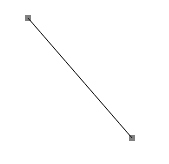
\includegraphics[height=5cm,width=\textwidth]{figures/bezier1.png}
			\caption{Lineal}
			\label{fig:bezier1}
	\end{subfigure}
	\begin{subfigure}[b]{.3\textwidth}
			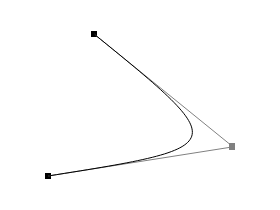
\includegraphics[height=5cm,width=\textwidth]{figures/bezier2.png}
			\caption{Cuadrática}
			\label{fig:bezier2}
	\end{subfigure}
	\begin{subfigure}[b]{.3\textwidth}
			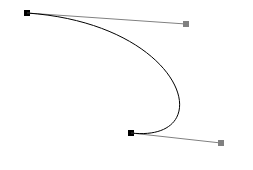
\includegraphics[height=5cm,width=\textwidth]{figures/bezier3.png}
			\caption{Cúbica}
			\label{fig:bezier3}
	\end{subfigure}
	\caption{Curvas de Bézier.}
	\label{fig:bezier}
\end{figure}

\begin{figure}[t]
	\centering	
	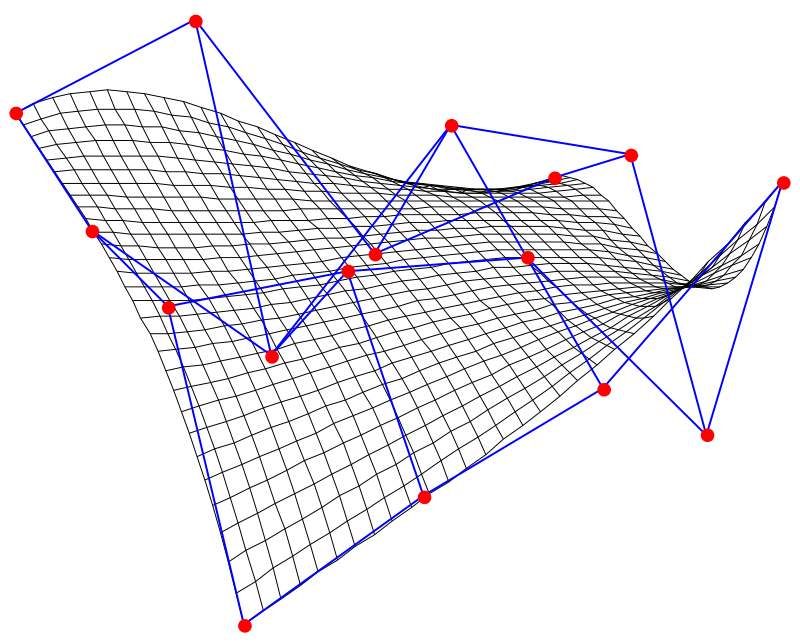
\includegraphics[height=8cm]{figures/beziersurface.png}
	\caption{Superficie de Bézier con 16 puntos de control}
	\label{fig:beziersurface}
\end{figure}

\section{Visualización de datos en 3D}
\label{ref:cloud}

Otra de las grandes áreas de la visualización científica es la de visualizar
conjuntos grandes de datos en tres dimensiones. Estos datos pueden ser tanto
escalares como vectoriales. Por ejemplo, se pueden monitorizar los datos de
temperatura en la atmósfera durante un determinado período de tiempo, queriendo
después visualizar las áreas que han estado más calientes de media. 

Otro tipo de visualización de datos en tres dimensiones es la visualización de
datos vectoriales en tres dimensiones, con el fin de capturar, por ejemplo,
flujos vectoriales de fluidos al rededor de un objeto, etc.

Para este tipo de tareas existen diferentes métodos de visualización, entre los
que se encuentran los siguientes:

\begin{itemize}
	\item Nubes de puntos (Figura~\ref{fig:pointcloud})
	\item Visualización de volumen (Figura~\ref{fig:volumevisualization})
	\item Isosuperficies (Figura~\ref{fig:isosurface})
	\item Planos cortados (Figura~\ref{fig:sliceplanes})
	\item Trazado de partículas (Figura~\ref{fig:particletracing})
	\item Visualización de vectores en 3D  (Figura~\ref{fig:vectorvisualization})
\end{itemize}

\begin{figure}[t]
	\centering
	\begin{subfigure}[b]{.45\textwidth}
			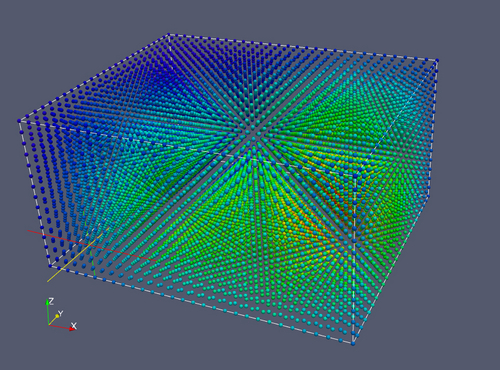
\includegraphics[height=6cm,width=\textwidth]{figures/pointcloud.jpg}
			\caption{Nube de puntos}
			\label{fig:pointcloud}
	\end{subfigure} \hfill
	\begin{subfigure}[b]{.45\textwidth}
			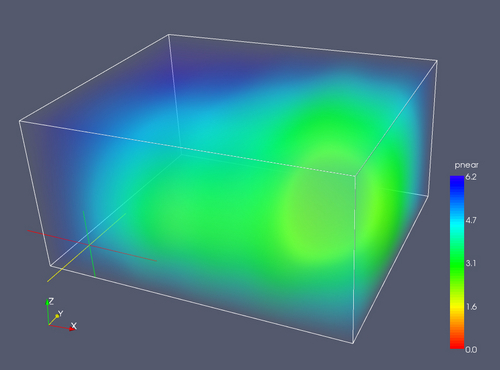
\includegraphics[height=6cm,width=\textwidth]{figures/volumevisualization.jpg}
			\caption{Visualización de volumen}
			\label{fig:volumevisualization}
	\end{subfigure}
	\newline \\
	\begin{subfigure}[b]{.45\textwidth}
			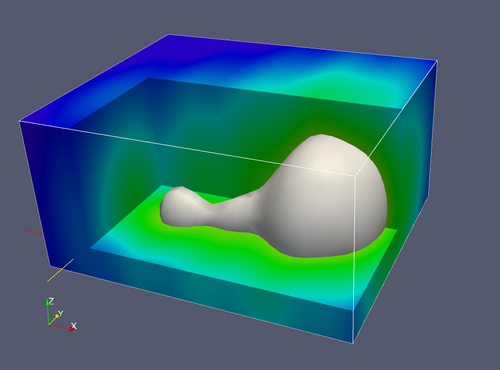
\includegraphics[height=6cm,width=\textwidth]{figures/isosurface.jpg}
			\caption{Isosuperficie}
			\label{fig:isosurface}
	\end{subfigure} \hfill
	\begin{subfigure}[b]{.45\textwidth}
			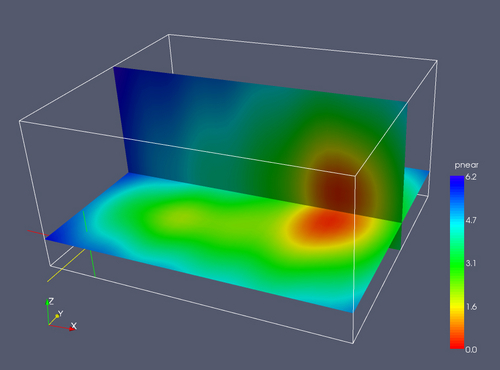
\includegraphics[height=6cm,width=\textwidth]{figures/sliceplanes.jpg}
			\caption{Planos cortados}
			\label{fig:sliceplanes}
	\end{subfigure}
	\newline\\
	\begin{subfigure}[b]{.45\textwidth}
			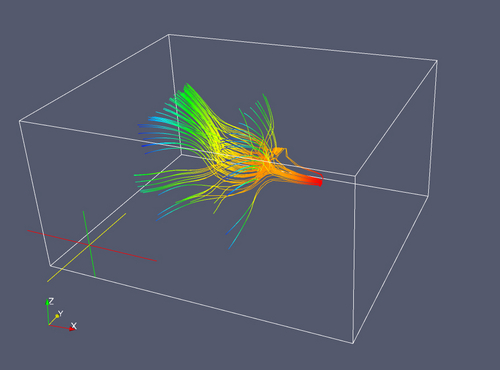
\includegraphics[height=6cm,width=\textwidth]{figures/particletracing.jpg}
			\caption{Trazado de partículas}
			\label{fig:particletracing}
	\end{subfigure} \hfill
	\begin{subfigure}[b]{.45\textwidth}
			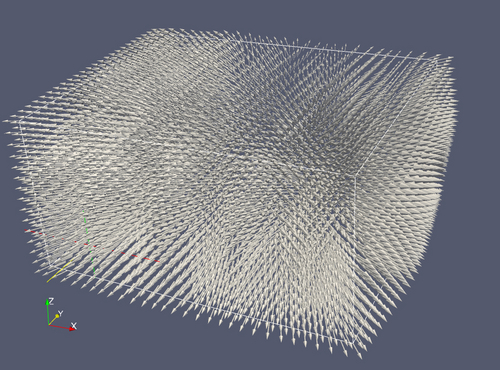
\includegraphics[height=6cm,width=\textwidth]{figures/vectorvisualization.jpg}
			\caption{Visualización de vectores}
			\label{fig:vectorvisualization}
	\end{subfigure}
	\caption{Técnicas de visualización en 3D. Figuras provenientes
	de~\cite{3dimages}}
	\label{fig:3dvis}
\end{figure}

\section{Sólidos de revolución}
\label{ref:revolution}

Los sólidos de revolución han sido siempre objeto de estudio en matemáticas,
física e ingeniería. Debido a la facilidad para calcular su área, son utilizadas
ampliamente en diseño industrial y modelado científico.

Este tipo de superficies surgen al rotar una curva planar ---la generatriz--- en
torno a un eje. Como se ha dicho antes, se conocen fórmulas exactas para su área
y volumen. Por ejemplo, cuando la revolución se produce en torno al eje $y$, se
tiene las ecuación~\eqref{eq:7} para el área, y la ecuación~\eqref{eq:8} para el
volumen del sólido encerrado por esta superficie. Sin embargo, si la revolución
se realiza en torno al eje x, las ecuaciones de área y volumen son~\eqref{eq:9}
y~\eqref{eq:10}.

\begin{equation} 
	A_y = 2\pi\int_{a}^{b}{x(t)\sqrt{\Big(\frac{dx}{dt}\Big)^2 +
		\Big(\frac{dy}{dt}\Big)^2}dt} \label{eq:7} 
\end{equation}

\begin{equation} 
		V = 2\pi\int_{a}^{b}{xf(x) dx} \label{eq:8} 
\end{equation}

\begin{equation} 
	A_y = 2\pi\int_{a}^{b}{y(t)\sqrt{\Big(\frac{dx}{dy}\Big)^2 +
		\Big(\frac{dy}{dt}\Big)^2}dt} \label{eq:9} 
\end{equation}

\begin{equation} 
		V = \pi\int_{a}^{b}{f(x)^2 dx} \label{eq:10} 
\end{equation}

\section{Coloreado de terrenos}
\label{ref:terrain}

Otro de los ejemplos típicos en visualización científica consiste en modelar un
terreno, ya sea en la Tierra o en otros planetas captando datos con sondas, y
colorearlo por alturas para hacerse una idea visual de lo que nos están diciendo
realmente esos datos. Un ejemplo de este coloreado de mapas puede verse en la
figura~\ref{fig:terrain}.

\begin{figure}[h!]
	\centering	
	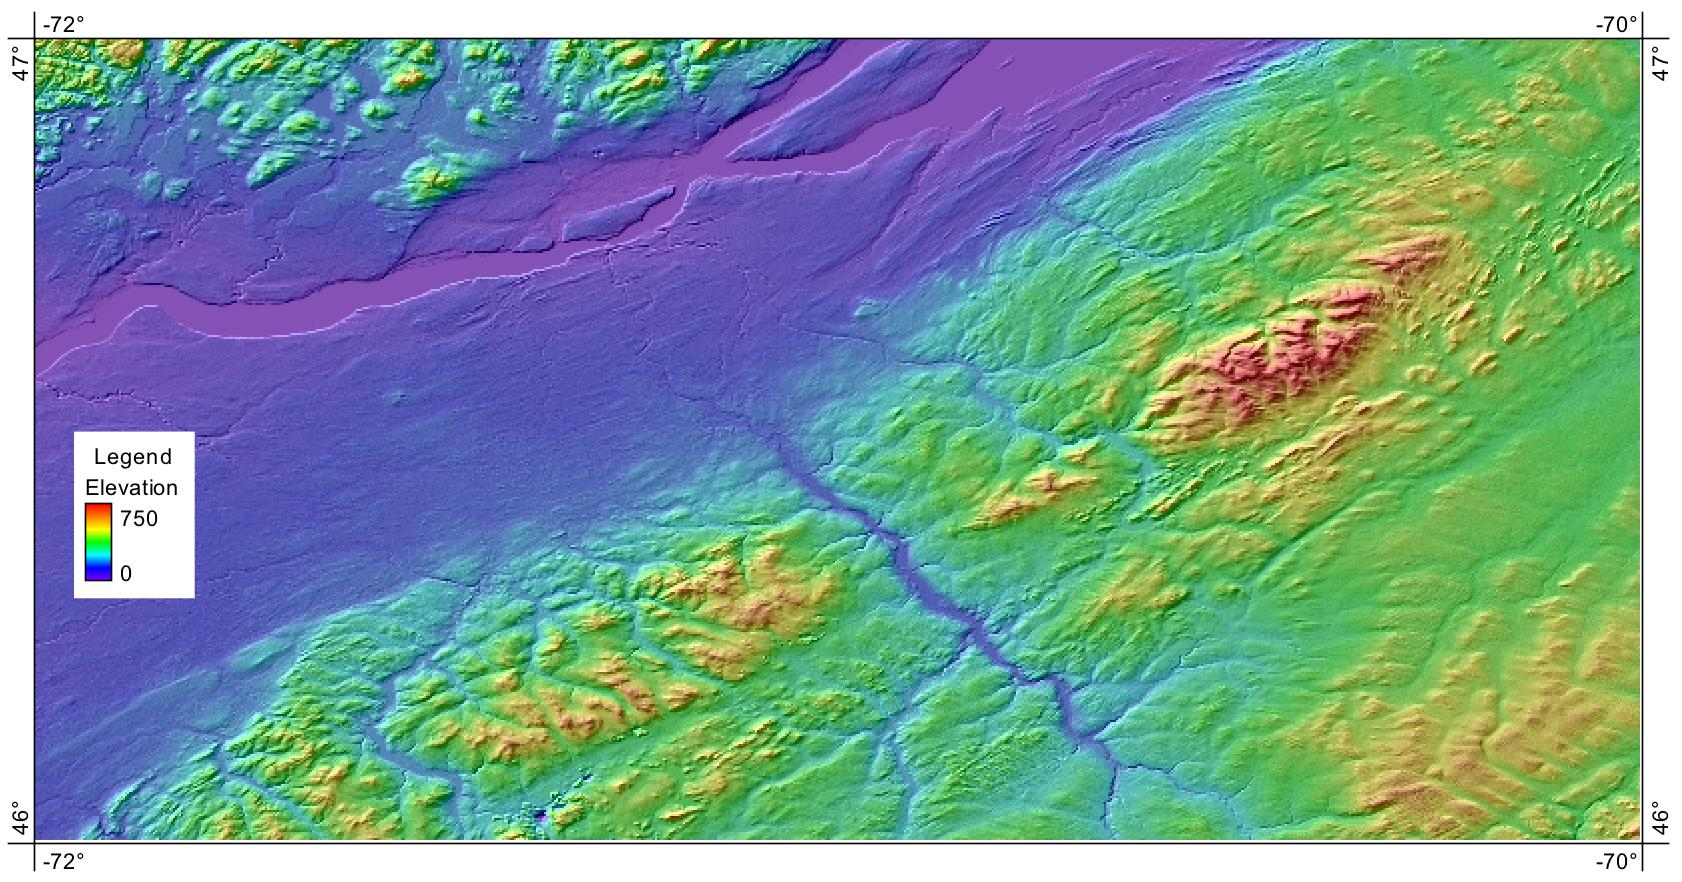
\includegraphics[height=8cm]{figures/terraincoloring.jpg}
	\caption{Coloreado de terreno por alturas}
	\label{fig:terrain}
\end{figure}

\section{Line Integral Convolution}
\label{ref:lic}

La última de las técnicas de visualización que vamos a ver tiene que ver con la
visualización de fluidos en dos dimensiones. Para ello veremos un método
importante denominado Line Integral Convolution.

El método Line Integral Convolution fue originalmente propuesto en el artículo
de~\citet{osti_10185520}. Se utiliza para visualizar campos vectoriales densos.
En este método, se utiliza una imagen junto con datos de un flujo vectorial,
modificando esta imagen para mostrar el flujo de los datos. (ver
Figura~\ref{fig:lic}). 

\begin{figure}[h!]
	\centering	
	\begin{subfigure}{.45\textwidth}
		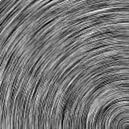
\includegraphics[height=5cm,width=\textwidth]{figures/lic2.png}
	\end{subfigure}
	\hfill
	\begin{subfigure}{.45\textwidth}
		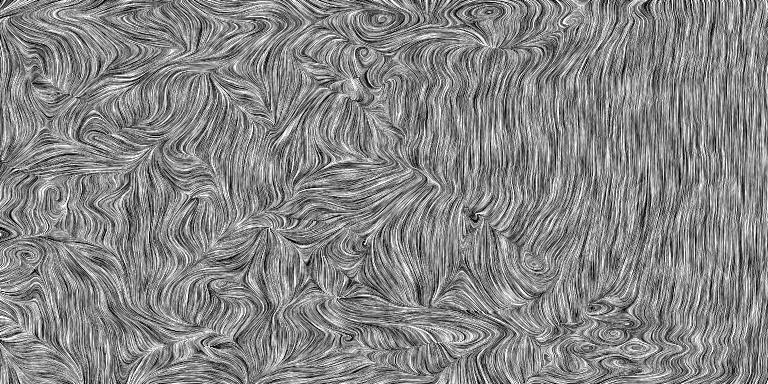
\includegraphics[height=5cm,width=\textwidth]{figures/lic1.png}
	\end{subfigure}
	\caption{Resultado del método Line Integral Convolution. Imagen
	de~\citet{osti_10185520}}
	\label{fig:lic}
\end{figure}

En~\citet{licthesis} se muestra como funciona el método de Line Integral
Convolution, señalando los principales pasos que sigue:

Para cada pixel en la imagen de entrada, hacer:
\begin{enumerate}
		\item Computar la línea de flujo \textit{(streamline)} para una longitud
				determinada por el usuario en direcciones positivas y
				negativas. (Figura~\ref{fig:licstreamline})
		\item \label{ref:licpaso2} Para cada punto en la streamline, computar su
				peso de convolución $h_i$. (Figura~\ref{fig:licweights})
		\item Computar el valor de salida del pixel con los valores de entrada y
				los pesos computados en~\ref{ref:licpaso2}.
				(Figura~\ref{fig:licoutputpixel})
\end{enumerate}

\begin{figure}
		\centering
		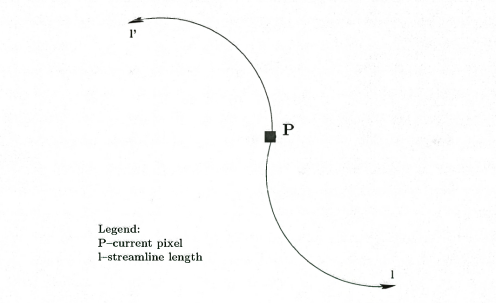
\includegraphics[height=9cm]{figures/licstreamline.png}
		\caption{Computar la línea de flujo. Imagen de~\citet{licthesis}}	
		\label{fig:licstreamline}
\end{figure}

\begin{figure}
		\centering
		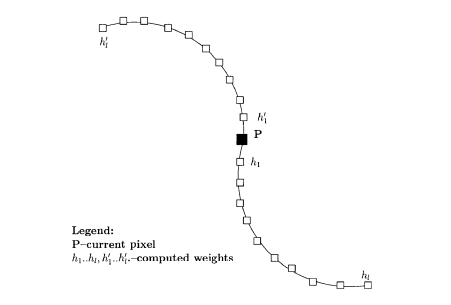
\includegraphics[height=9cm]{figures/licweights.png}
		\caption{Computar los pesos. Imagen de~\citet{licthesis}}	
		\label{fig:licweights}
\end{figure}

\begin{figure}
		\centering
		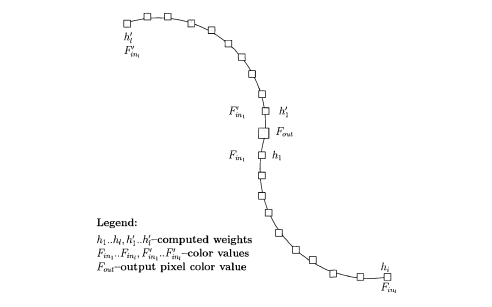
\includegraphics[height=9cm]{figures/licoutputpixel.png}
		\caption{Computar valores de salida del pixel. Imagen de~\citet{licthesis}}	
		\label{fig:licoutputpixel}
\end{figure}

Como imagen de entrada se puede utilizar, realmente, cualquier imagen,
haciendo ver las líneas de flujo con los colores de la imagen original. Sin
embargo, con el fin de que perturbaciones en la imagen original no condicionen
el análisis del flujo a visualizar, la opción recomendada y casi siempre
utilizada en este método es la del ruido blanco, debido a la distribución
uniforme de los colores de sus píxeles. 

\subsection{Computar la línea de flujo}
\label{ref:streamline}

Para computar la línea de flujo se ha de utilizar algún método numérico. Entre
las posibilidades se encuentran el método de Euler, utilizado
por~\citet{licthesis}, el método de Euler de paso variable, utilizado por los
autores originales en~\citet{osti_10185520}, o el método de Runge-Gutta de orden
4, propuesto como alternativa en ambos textos. En la
sección~\ref{makereference5.4.3}, se explican estos métodos como preparación
para su implementación. De esta manera, se consiguen una serie de puntos a lo
largo de la línea de flujo, dependiendo del paso escogido en el método numérico
y la longitud de la línea escogida por el usuario.

\subsection{Computar los pesos de convolución}
\label{ref:convolution}

Este paso consiste en encontrar la integral exacta del núcleo de convolución $k$
en cada punto de la línea de flujo computado en el paso anterior. Es decir, se
ha de resolver la integral~\eqref{eq:11}.

\begin{equation}
		h_i = \int_{a}^{b}k(\omega) d\omega \label{eq:11}
\end{equation}

donde $i$ se representa el índice del punto actual en la línea de flujo, $a$
es la distancia a lo largo de la línea de flujo entre el punto actual y el pixel
para el que queremos calcular el valor de salida y $b$ es igual a $a$ más el
tamaño del paso utilizado en el paso actual $\Delta s_i$. Más información acerca
del núcleo de convolución puede encontrarse en~\citet{osti_10185520}.

\subsection{Computar los valores de salida del pixel}
\label{ref:salida}

Para calcular los valores de salida del pixel una vez calculados los pesos de
los puntos de la línea de flujo, se sigue la siguiente ecuación:

\begin{equation}
		F_{out}(x,y) =
		\frac{\sum\limits_{i=0}^{l}{F_{in}(P_i)h_i}+\sum\limits_{i=0}^{l'}{F_{in}(P'_i)h'_i}}{\sum\limits_{i=0}^{l}{h_i} + \sum\limits_{i=0}^{l'}{h'_i}} \label{eq:12}
\end{equation}

\cleardoublepage

\chapter{Aplicación desarrollada}
\label{makereference5}

En este capítulo se introducirá la aplicación que se ha desarrollado con el
fin de demostrar los conceptos expuestos en los capítulos anteriores. En
concreto se desarrollarán shaders para los siguientes problemas:

\begin{itemize}
		\item Coloreado de terrenos
		\item Curvas de Bézier
		\item Superficies de Bézier
		\item Sólidos de revolución
		\item Nubes de puntos
		\item Negativo de una imagen
		\item Detección de bordes en una imagen
		\item Line Integral Convolution
\end{itemize}

Para el desarrollo de la aplicación y los shaders será necesario introducir
algunos conceptos matemáticos importantes, que se explican en la
sección~\ref{makereference5.1}.

\section{Plan de desarrollo}
\label{makereference5.1}

Durante las primera semanas de desarrollo de la aplicación lo más importante fue
realizar un exhaustivo estudio del funcionamiento de OpenGL, así como la lectura
y realización de tutoriales sobre la materia. Una vez adquirido el conocimiento
necesario, se comenzó a desarrollar el esqueleto principal de la aplicación,
sobre el cual se incorporarían después los distintos tipos de visualización a
realizar.

Una vez desarrollado este esqueleto se comenzó a la preparación de los shaders
que se utilizarían en cada uno de los problemas, para lo que se utilizó en gran
medida la información expuesta en el texto~\citet{Bailey}.

El siguiente paso fue conseguir datos y prepararlos adecuadamente para poder
mostrar las capacidades de visualización de la aplicación, así como comprobar su
correcto funcionamiento.

Lo anterior fue reiterado con cada uno de los problemas, añadiéndose cada vez
más a lo largo del desarrollo de todo el proyecto.

\section{Herramientas de desarrollo}
\label{makereference5.2}

Como entorno de desarrollo principal se ha utilizado el sistema operativo Ubuntu
Linux 18.04 LTS~\cite{UBUNTU}. En este sistema, además, se han utilizado las
siguientes herramientas de desarrollo:

\begin{itemize}
		\item Vim como editor de textos.~\cite{VIM}
		\item Git para el control de versiones.~\cite{GIT}
		\item Github como respositorio.~\cite{GITHUB}
		\item GCC como compilador.~\cite{GCC}
		\item GDB para la depuración.~\cite{GDB}
		\item Make para la gestión de dependencias.~\cite{MAKE}
\end{itemize}. 

Asimismo, siguiendo las recomendaciones del tutorial~\citet{LearnOpenGL}, se han
utilizado las siguientes librerías:

\begin{itemize}
		\item GLFW~\cite{GLFW}. GLFW es una librería orientada específicamente a
				OpenGL que proporciona las necesidades básicas para el
				renderizado en pantalla. Permite crear un contexto de OpenGL,
				definir parámetros de ventana y manejar la entrada del usuario.
				Estas son las funciones que utilizaremos en la aplicación.
		\item GLAD~\cite{GLAD}. La localización de funciones de OpenGL depende
				tanto del controlador gráfico utilizado como del sistema
				operativo utilizado. Esta localización es desconocida en tiempo
				de  compilación y ha de ser conseguida en tiempo de ejecución.
				Es, pues, tarea del programador conseguir la localización de
				estas funciones. GLAD es una  librería que realiza esta tarea
				automáticamente.
		\item Assimp~\cite{ASSIMP}. Assimp --- \textit{The
				Open-Asset-Importer-Lib} --- es una librería que permite
				importar diferentes formatos de modelos 3D de una manera
				uniforme. Será utilizado para cargar los modelos para el
				colorado de terrenos.
		\item GLM~\cite{GLM}. GLM --- OpenGL Mathematics --- es una librería
				para matemáticas en software gráfico en C++ basada en las
				especificaciones del lenguaje GLSL. Proporciona funciones
				diseñadas e implementadas con el mismo convenio de nombres y
				funcionalidades que GLSL. Proporciona capacidades como
				transformaciones de matrices, cuaterniones, empaquetado de
				datos, aleatoriedad, ruido\ldots
		\item Otras librerías especificas del sistema operativo, como Pthreads,
				xrandr, x11, xi, xcursor, etc.
\end{itemize}

\section{Diseño de la aplicación}
\label{makereference5.3}

Para esta aplicación se ha optado por un diseño modular orientado a objetos, en
el que poder incrementalmente añadir distintos tipos de visualización sin tener
demasiados problemas. Como se ha expuesto en la sección~\ref{makereference5.1}
la aplicación consta de un esqueleto principal utilizado por todos los tipos de
visualización. Este esqueleto consta de una ventana principal, creada en el
programa principal, en la que se renderizará el objeto particular que representa
el tipo de visualización. Así, con el fin de añadir un nuevo tipo de
visualización solo se habrían de realizar las siguientes acciones:

\begin{enumerate}
		\item Crear un nuevo objeto que implemente los métodos necesarios
				de la clase \verb|Object|.
		\item Añadir un nuevo modo al \verb|enum Modes|.
		\item Añadir las opciones necesarias para dicho objeto en el programa
				principal e incluir la nueva clase \verb|#include "class.h"|.
		\item Actualizar las dependencias en el Makefile.
\end{enumerate}

En esta ventana principal se tiene por defecto un sistema de cámara en primera
persona, con la capacidad de moverse para visualizar mejor detalles del objeto
en cuestión. Este sistema puede ser sobreescrito en el objeto específico en
caso de necesitar otro comportamiento. 

En la clase \verb|Object| existen tres métodos virtuales puros, que han de ser
implementados por las clases específicas de cada tipo de visualización:


\begin{itemize}
		\item \verb|draw()|, que ha de encargarse de dibujar el objeto en
				cuestión.
		\item \verb|processInput(GLFWwindow * window)|, que ha de especificar que
				hacer con la entrada del usuario para este tipo de
				visualización.
		\item \verb|setUniforms()|, que ha de especificar las variables
				\verb|uniform| que utilicen los shaders de este tipo de
				visualización.
\end{itemize}

Estos métodos se llaman una vez por vuelta del bucle principal. En la sección
siguiente se introducen las matemáticas necesarias e importantes para el
desarrollo de la aplicación y los shaders concretos.

\section{Matemáticas necesarias}
\label{makereference5.4}

Con el fin de desarrollar el sistema de cámaras que utiliza la aplicación es
necesario conocer varios conceptos importantes sobre álgebra, geometría lineal y
transformaciones matriciales, así como los ángulos de Euler y su relación con
los cuaterniones. También se explorarán distintos métodos numéricos, relevantes
en el método de Line Integral Convolution, así como fórmulas matemáticas
específicas de cada tipo de visualización.

\subsection{Transformaciones matriciales}
\label{makereference5.4.1}

Como vamos a trabajar con objetos tridimensionales y una cámara móvil,
necesitamos realizar transformaciones sobre los vértices que componen nuestros
objetos para que estos aparezcan en su lugar y con sus dimensiones adecuadas.
Es deseable, además, realizar estas operaciones con vectores matricialmente,
puesto que éstas permiten presentar transformaciones arbitrarias en un
formato consistente y apto para la computación. Así, se pueden concatenar
diferentes transformaciones de manera sencilla multiplicando sus matrices. 

Entre estas transformaciones podemos encontrar lineales y no lineales. Así, para
representar matricialmente transformaciones no lineales en un espacio Euclídeo
$n$-dimensional $\mathbb{R}^n$ se puede utilizar una transformación lineal en el
espacio $(n+1)$-dimensional $\mathbb{R}^{n+1}$. Este tipo de transformaciones
incluye tanto las transformaciones afines como transformaciones proyectivas.

Esta es la razón por la que las matrices $4 \times 4$ son tan ampliamente
utilizadas en la informática gráfica y, en consecuencia, en nuestra
aplicación.

En esta sección se presentan las transformaciones lineales y afines más
habituales y necesarias para nuestra aplicación, así como sus formas
matriciales. 

\subsubsection{Traslación}
\label{makereference5.4.1.1}

Se denomina traslación a la operación consistente en \textit{mover} un vector en
una posición a otra nueva posición. Supongamos, pues, que queremos trasladar un
vector $\overrightarrow{v} = (x,y,z)$ en la dirección marcada por el vector
$\overrightarrow{t} = (t_1, t_2, t_3)$ como se muestra en la
figura~\ref{fig:traslation}. Para ello realizaríamos la siguiente operación:

\begin{figure}
	\centering	
	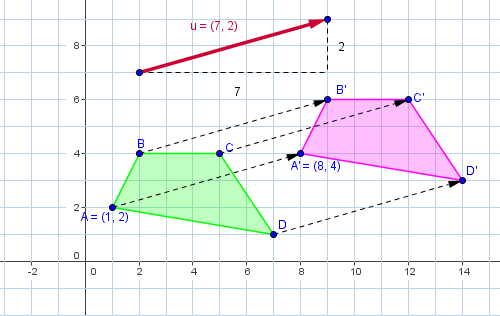
\includegraphics[height=9cm]{figures/traslacion.png}
	\caption[Traslación de un vector.]{Traslación de un vector.
	Fuente:~\cite{vectortraslationimage}}
	\label{fig:traslation}
\end{figure}

\begin{equation}
	\label{eq:translation}
	\overrightarrow{v}' = \overrightarrow{v} + \overrightarrow{t} = 
	\left( \begin{array}{c}
			x + t_1 \\
			y + t_2 \\
			z + t_3 \\
	\end{array} \right)
\end{equation}

La traslación se trata de una transformación afín sin puntos fijos. Como se ha
expuesto previamente, para poder representar esta transformación de forma
matricial se ha de recurrir a un espacio de una dimensión más. Por tanto, se
recurre a las coordenadas homogéneas para representar la traslación de un
espacio vectorial con multiplicación de matrices. Escribiendo el vector
$\overrightarrow{v} = (x,y,z)$ utilizando una cuarta coordenada homogénea
$\overrightarrow{v} = (x,y,z,1)$. Esta operación se muestra
en~\eqref{eq:matrixtranslation}. 

\begin{equation}
	\label{eq:matrixtranslation}
	\overrightarrow{v}' = 
	\left( \begin{array}{cccc}
			1 & 0 & 0 & t_1 \\
			0 & 1 & 0 & t_2 \\
			0 & 0 & 1 & t_3 \\
			0 & 0 & 0 & 1 \\
	\end{array} \right)
	\left( \begin{array}{c}
			x \\
			y \\
			z \\
			1 \\
	\end{array} \right) = 
	\left( \begin{array}{c}
			x + t_1 \\
			y + t_2 \\
			z + t_3 \\
			1 \\
	\end{array} \right)
\end{equation}\\

\subsubsection{Escalado}
\label{makereference5.4.1.2}

El escalado de un vector es la operación consistente en modificar la longitud
del vector. Para ello, debemos multiplicar cada una de sus coordenadas por el
factor de escalado deseado en cada eje. Es decir, para escalar un vector
$\overrightarrow{v}$ por un factor de $0.5$ en el eje $x$ y $3$ en el eje $y$,
la operación a realizar sería la siguiente:

\begin{equation}
	\label{eq:scaling}
	\overrightarrow{v} = 
	\left( \begin{array}{c}
			2 \\
			3 \\
	\end{array} \right)
	\;\;\;\;\;
	\overrightarrow{v}' =
	\left( \begin{array}{c}
		2\cdot0.5 \\
		3\cdot3 \\
	\end{array}	\right) =  
	\left( \begin{array}{c}
			1 \\
			9 \\
	\end{array} \right)
\end{equation}\\

\begin{figure}[h]
	\centering
	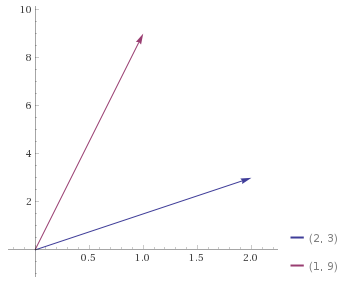
\includegraphics{figures/scaling.png}
	\caption[Escalar un vector.]{Escalar un vector. Fuente:~\cite{wolfram}}
	\label{fig:scaling}
\end{figure}

Esta operación de escalado se puede escribir matricialmente como sigue.
Supongamos que tenemos un vector $\overrightarrow{v}=(x,y,z)$ y lo queremos
escalar por un factor $fac=(F_1,F_2,F_3)$. Entonces podemos escribir la
operación anterior con la matriz $FAC$ como sigue:

\begin{equation}
	\label{eq:matrixscaling}
	\overrightarrow{v}' = 
	\left( \begin{array}{cccc}
			F_1 & 0   & 0   & 0	\\
			0   & F_2 & 0   & 0	\\
			0   & 0   & F_3 & 0	\\
			0   & 0   & 0   & 1	\\
	\end{array} \right)
	\left( \begin{array}{c}
			x \\
			y \\
			z \\
			1 \\
	\end{array} \right) =
	\left( \begin{array}{c}
			F_1\cdot x \\
			F_2\cdot y \\
			F_3\cdot z \\
			1 \\
	\end{array} \right)
\end{equation}\\

Nótese que también en este caso al vector $\overrightarrow{v}$ se le ha añadido
una cuarta coordenada $w$ con el fin de ser consistentes con aquellas
transformaciones no lineales que necesitan de un espacio de dimensión mayor. 

\subsubsection{Rotación}
\label{makereference5.4.1.3}

Al contrario de los casos de la rotación y traslación de vectores expuestas
anteriormente, el caso de la rotación requiere un estudio más profundo en el
caso tridimensional para la matemática aplicada. Por esto, se dedica una sección
exclusiva para este tema. (Ver sección~\ref{makereference5.4.2}).

\subsection{Rotación: Ángulos de Euler y Cuaterniones}
\label{makereference5.4.2}

La rotación tridimensional es un caso particularmente complejo. Esto se debe a
determinados problemas que surgen a la hora de formalizar matemáticamente este
movimiento. 

La manera más intuitiva de pensar en la rotación consiste en especificar esta
rotación mediante un eje de giro y un ángulo. Con esto, el movimiento
consistiría en rotar el vector en torno al eje de giro. (Ver
Figura~\ref{fig:rotacion}). 

Existen diversas maneras de formular matemáticamente este movimiento. Para ello
existe un grupo, llamado $SO(3)$, que es el grupo de todas las rotaciones en
torno al origen del espacio vectorial Euclídeo $\mathbb{R}^3$ bajo la operación
de la composición. Una rotación en $\mathbb{R}^3$ es una aplicación lineal. Como
toda aplicación lineal en un espacio vectorial, ésta puede ser representada
mediante una matriz, dando lugar a la representación matricial de la rotación.

\begin{figure}
	\centering		
	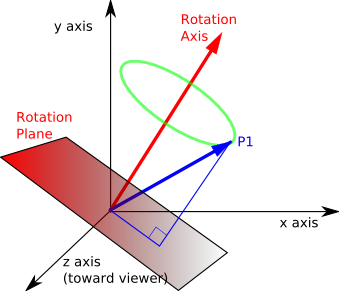
\includegraphics[height=10cm]{figures/rotation.png}
	\caption[Rotación de un vector 3D.]{Rotación de un vector 3D.
	Fuente:~\cite{rotationimage}}
	\label{fig:rotacion}
\end{figure}

\subsubsection{Ángulos de Euler y Matriz de rotación}
\label{makereference5.4.2.1}

En el espacio vectorial $\mathbb{R}^3$, los vectores se representan a partir de
una base. Esta base estará formada por tres vectores unitarios. Por tanto, si
queremos realizar una rotación de cualquier otro vector en $\mathbb{R}^3$,
bastará con rotar los vectores de la base acorde al eje de rotación y después
calcular el vector a rotar en términos de la base rotada. 

Los vectores rotados que forman la nueva base definen completamente la rotación
y, escritos como una matriz nos da la matriz de rotación. Esta matriz, al ser
los vectores una base ortonormal de $\mathbb{R}^3$, forman una matriz ortogonal.
Por tanto, el grupo $SO(3)$ se identifica con el grupo formado por las matrices
ortogonales $3\times 3$ bajo la operación de la multiplicación. Estas matrices
se conocen como \textit{Matrices Ortogonales Especiales (Special Orthogonal
Matrices)}, de ahí la notación de $SO(3)$. 

Como sabemos, dos rotaciones en $SO(3)$ se pueden concatenar mediante la
composición, dando lugar a otra nueva rotación. Lo mismo pasa con la
representación matricial, multiplicando dos matrices de rotación. Para nuestra
aplicación, es conveniente realizar las rotaciones como composición de
rotaciones en torno a los ejes de referencia. Para ello definimos las matrices
de rotación. 

\begin{equation}
	R_x(\theta) =
	\left(	
		\begin{array}{cccc}
			1 & 0 & 0 & 0 \\				
			0 & \cos{\theta} & -\sin{\theta} & 0 \\				
			0 & \sin{\theta} & \cos{\theta} & 0 \\				
			0 & 0 & 0 & 1 \\				
		\end{array}
	\right)
\end{equation}

\begin{equation}
	R_y(\theta) =
	\left(	
		\begin{array}{cccc}
			\cos{\theta} & 0 & \sin{\theta} & 0 \\				
			0 & 1 & 0 & 0 \\				
			-\sin{\theta} & 0 & \cos{\theta} & 0 \\				
			0 & 0 & 0 & 1 \\				
		\end{array}
	\right)
\end{equation}

\begin{equation}
	R_z(\theta) =
	\left(	
		\begin{array}{cccc}
			\cos{\theta} & -\sin{\theta} & 0 & 0 \\				
			\sin{\theta} & \cos{\theta} & 0 & 0 \\				
			0 & 0 & 1 & 0\\				
			0 & 0 & 0 & 1 \\				
		\end{array}
	\right)
\end{equation} 

Esto da lugar a los conocidos como ángulos de Euler, llamados en inglés
\textit{yaw, pitch, roll}. (Ver Figura~\ref{fig:eulerangles}). Así, una rotación
cualquiera en el espacio tridimensional viene dada por:

\begin{figure}
	\centering
	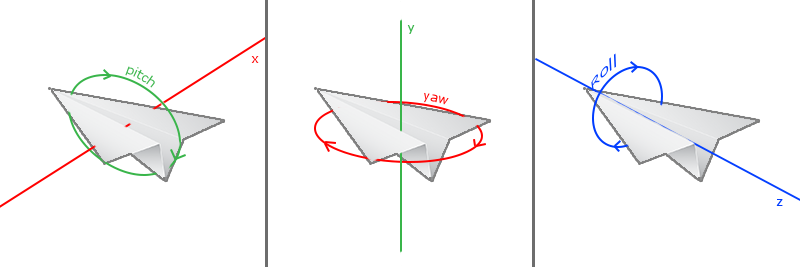
\includegraphics[height=7.5cm,width=\textwidth]{figures/eulerangles.png}
	\caption[Ángulos de Euler.]{Ángulos de Euler. Fuente:~\citet{LearnOpenGL}}
	\label{fig:eulerangles}
\end{figure}

\begin{equation}
		R = Roll(\phi)Pitch(\theta)Yaw(\varphi) = R_x(\phi)R_y(\theta)R_z(\varphi)	
\end{equation}

Ahora bien, aunque este sistema es el que utilizaremos en nuestra aplicación,
tanto mediante GLM como implementándolo nosotros, existen diversos problemas
derivados de él. El más importante es el llamado Bloqueo del
Cardán~\cite{Vince:2011:QCG:2016678}. Aunque los formalismos matemáticos son más
complejos, intuitivamente este bloqueo ocurre debido a que la descripción de
cualquier rotación tridimensional mediante ángulos de Euler no es única y
existen puntos sobre los que no todo cambio en el espacio de rotaciones puede
ser expresado mediante cambios en el espacio de los ángulos de Euler. 

Con el fin de disminuir el riesgo del bloqueo, se puede prescindir de la
multiplicación de matrices utilizando una sola matriz utilizando un eje de giro
arbitrario unitario $u = (u_x, u_y, u_z)$ y un ángulo de giro $\theta$. La
procedencia de dicha matriz se puede consultar en~\citet{Rodrigues}. 

\begin{equation}
		R = 
		\left(
				\begin{array}{cccc}
						\cos\theta + u_x^2(1-\cos\theta) &
						u_xu_y(1-\cos\theta)-u_z\sin\theta &
						u_xu_z(1-\cos\theta)+u_y\sin\theta & 0 \\

						u_yu_x(1-\cos\theta)+u_z\sin\theta & \cos\theta +
						u_y^2(1-\cos\theta) &
						u_yu_z(1-\cos\theta)-u_x\sin\theta & 0 \\

						u_zu_x(1-\cos\theta)-u_y\sin\theta &
						u_zu_y(1-\cos\theta) + u_x\sin\theta & \cos\theta +
						u_z^2(1-\cos\theta) & 0 \\

						0 & 0 & 0 & 1 \\
				\end{array}
		\right)
\end{equation}

\subsubsection{Cuaterniones}
\label{makereference5.4.2.2}

Debido a la importancia de la precisión en muchos sistemas informáticos que
necesitan cálculos de rotaciones y el problema que supone el bloqueo del Cardán,
se hace importante la mención de los cuaterniones como sistema de representación
de rotaciones en tres dimensiones, aunque no los vayamos a utilizar en nuestra
aplicación. 

Los cuaterniones, también conocidos como cuaternios, suponen una notación para
representar orientaciones y rotaciones en tres dimensiones. En contraposición
con los ángulos de Euler, son más sencillos de componer y previenen el bloqueo
del Cardán. Comparados con las matrices de rotación, suponen un método más
compacto, más estable numéricamente y más eficiente. 

Los cuaterniones son una extensión de los números complejos, descritos por
primera vez por William Rowan Hamilton en 1843, definiéndolos como el cociente
de dos lineas dirigidas en un espacio tridimensional.  Cuando se utilizan para
representar rotaciones se les denomina también cuaterniones de rotación, puesto
que representan el grupo $SO(3)$. 

Generalmente, se representan de la siguiente forma:

\[a + b\boldsymbol{i} + c\boldsymbol{j} + d\boldsymbol{k} \] 

donde $a,b,c$ y $d$ son números reales y $\boldsymbol{i}, \boldsymbol{j}$ y
$\boldsymbol{k}$ son las unidades fundamentales del cuaternión. Además, los
cuaterniones  siguen las reglas algebraicas usuales, excepto la de la propiedad
conmutativa de la multiplicación, y cumplen la siguiente propiedad:

\[\boldsymbol{i}^2 = \boldsymbol{j}^2 = \boldsymbol{k}^2 = \boldsymbol{ijk} = -1 \]

Es conveniente verlos representados como un escalar más un vector, es decir:

\[a + b\boldsymbol{i} + c\boldsymbol{j} + d\boldsymbol{k} = a +
\overrightarrow{v} \] 

considerando la parte imaginaria $b\boldsymbol{i} + c\boldsymbol{j} +
d\boldsymbol{k}$ como un vector $\overrightarrow{v} = (b,c,d)$. 

Recordemos que cualquier rotación en el espacio tridimensional puede verse como
una giro de ángulo $\theta$ en torno a un eje definido por un vector unitario
$u$. Esto puede ser representado mediante un cuaternión de la siguiente forma:

\[\boldsymbol{q} = \exp{\frac{\theta}{2}(u_x\boldsymbol{i} + u_y\boldsymbol{j} +
		u_z\boldsymbol{k})} = \cos{\frac{\theta}{2}} + (u_x\boldsymbol{i} + 
u_y\boldsymbol{j} + u_z\boldsymbol{k})\sin{\frac{\theta}{2}} \]

Se puede demostrar que un la rotación deseada se puede aplicar a un vector
ordinario $\boldsymbol{p} = (p_x, p_y, p_z) = p_x\boldsymbol{i} +
p_y\boldsymbol{j} + p_z\boldsymbol{k}$ en el espacio tridimensional, considerado
como un cuaternión con parte real igual a cero, evaluando la conjunción de
$\boldsymbol{p}$ por $\boldsymbol{q}$:

\[ \boldsymbol{p'} = \boldsymbol{qpq^{-1}} \]

donde $\boldsymbol{p'}$ es la nueva posición del vector $\boldsymbol{p}$ tras la
rotación. La parte vectorial del este cuaternión es el vector deseado. Se puede
leer más acerca de cuaterniones utilizados para las rotaciones en~\citet{Vicci}.

\subsection{Métodos Numéricos para la resolución de Ecuaciones Diferenciales} 
\label{makereference5.4.3}

Como ya se vio en la sección~\ref{ref:lic}, en el método del Line Integral
Convolution se ha de utilizar un método numérico para computar la línea de
flujo. En esta sección se analizan algunos de los métodos utilizados y
propuestos tanto por~\citet{osti_10185520} como por \citet{licthesis}.

Para poder analizar los métodos hemos de introducir algunas definiciones
relacionadas con ellos. Recordemos que un método numérico sirve para calcular de
manera aproximada la solución de una ecuación diferencial en un intervalo $[t_0,
T]$. Para ello, dividiremos el intervalo en una serie de puntos, dando lugar a
los siguientes conceptos~\cite{ANNU}:

\begin{itemize}

		\item \textbf{Puntos de red.} Cada uno de los puntos en los que se
				divide el intervalo $[t_0, T]$. Los subintervalos resultantes
				pueden ser de longitud constante (Redes uniformes de paso
				$h=\frac{T-t_0}{N}$) o de longitud variable, dando lugar a
				los métodos númericos de paso variable.

		\item \textbf{Esquema Numérico.} Se denomina esquema numérico al proceso
				iterativo mediante el cual, conociendo los $r$ primeros valores
				$x_0, x_1, \ldots, x_{r-1}$, que son aproximaciones de los
				valores exactos $x(t_0),x(t_1),\ldots,x(t_{n-1})$ de la solución
				de la ecuación diferencial en los puntos $t_0, t_1, \ldots,
				t_{r-1}$ podemos calcular todos los demás valores $x_n, n =
				r,\ldots,N$, que son aproximaciones de los valores exactos en
				los puntos de red.

				El esquema numérico se escribe de la siguiente forma:

				\begin{equation}
					\left\{ \begin{aligned}
							& x_0,x_1,\ldots,x_{r-1} \; \textrm{dados} \\
							& x_{n-r} = \Phi
							(t_n,x_n,x_{n+1},\ldots,x_{n+r-1},h), \; n =
							0,\ldots,N-r \\
					\end{aligned} \right.
				\end{equation}

		\item \textbf{Error Local de Truncamiento.} Dado un esquema como el
				anterior, suponiendo que las soluciones exactas verifican

				\begin{equation}
						x(t_{n+r}) = \Phi (t_n,
						t_{n+1},\ldots,t_{n+r-1},x(t_n),x(t_{n+1}),\ldots,x(t_{n+r-1}))
						+ h\tau_{n+r}(h)
				\end{equation}

				el error local de truncamiento viene dado por

				\begin{equation}
						\tau (h) := \max_{n=0,\ldots,N-r}|\tau_{n+r}(h)|	
				\end{equation}

				que consiste en el error que se comete al calcular el valor
				exacto utilizando el esquema numérico.

		\item \textbf{Consistencia.} Se dice que un método es consistente si

				\begin{equation}
						\lim_{h\to 0} \tau(h) = 0	
				\end{equation}

				Se dice que es consistente de orden $p$ si

				\begin{equation}
					\tau(h) = O(h^p)				
				\end{equation}

		\item \textbf{Error Global de Discretización.} Siguiendo la notación
				anterior, el Error global de discretización viene dado por

				\begin{equation}
					\epsilon (h) := \max_{n=0,\ldots,N}|x_n - x(t_n)|
				\end{equation}

		\item \textbf{Convergencia.} Se dice que un método es convergente cuando
				se verifica lo siguiente:

				\begin{equation}
						si \;\;\; \max_{k=0,\ldots,r-1}|x_k - x(t_k)|
						\xrightarrow {h\to 0} 0	\;\;\; entonces \;\;\; \lim_{h\to
						0}\epsilon(h) = 0
				\end{equation}

				Se dice que es convergente de orden $p$ si

				\begin{equation}
						\epsilon(h) = O(h^p)	
				\end{equation}

\end{itemize}

Con estas nociones ya podemos empezar a analizar los distintos métodos
utilizados, para así conocer cuáles proporcionarán mejores resultados. 

\subsubsection{Método de Euler}
\label{makereference5.4.3.1}

El método de Euler es el más sencillo de los métodos numéricos a considerar. Se
trata de un método por aproximación de la derivada. Para ver cómo aparece este
método, hemos de recurrir a la definición de derivada. Para cada $t \in (t_0,T)$

\begin{equation}
		x'(t) = \lim_{h \to 0} \frac{x(t+h) - x(t)}{h} 	
\end{equation}

Si $h>0$ es suficientemente pequeño, podemos suponer que

\begin{equation}
		x'(t_n)\approx \frac{x(t_n+h) - x(t_n)}{h} = \frac{x(t_{n+1}) -
		x(t_n)}{h}	
\end{equation}

lo que nos conduce a que

\begin{equation}
		x(t_{n+1}) \approx x(t_n) + hf(t_n,x(t_n))	
\end{equation}

De aquí aparece el esquema numérico del método de Euler

\begin{equation}
		\left\{ \begin{aligned}
				& x_{n+1} = x_n + hf(t_n,x_n) \; n=0,\ldots,N-1 \\
				& x_0 \approx a \\
		\end{aligned} \right.
\end{equation}

En~\citet{ANNU} se puede ver una demostración de que el método de Euler supone
un método \textbf{consistente de orden 1} y \textbf{convergente}.

\subsubsection{Método de Euler de paso variable}
\label{makereference5.4.3.2}

El método de Euler de paso variable sigue la misma idea general que el método de
Euler de paso uniforme. En este caso, sin embargo, el siguiente punto en el que
calcular la solución aproximada se calcula en cada paso. Para ello, se ha de
fijar previamente una tolerancia permitida para el error cometido. Por tanto,
necesitamos ser capaces de \textbf{estimar} el error que vamos a cometer al
escoger el siguiente paso. Entonces, si el error estimado es mayor que la
tolerancia fijada, el cálculo se descarta y se vuelve a realiza, y si éste es
menor que la tolerancia, entonces se acepta y se pasa al siguiente cálculo.

Con el fin de realizar esta estimación, como hemos dicho, necesitamos introducir
los siguientes conceptos:

\begin{itemize}

		\item \textbf{Error local relativo al paso $h$.} Se define el error local relativo
				al paso $h$ en el nodo $t_{n+1} = t_n + h$ como 

				\begin{equation}
						ERR_n(h) := \frac{|y(t_n + h) - y_1(t_n,h)|}{h}	
				\end{equation}

				donde la función $y = y(t)$ es la solución del problema y la
				función $y_1(t_n,h)$ representa la aproximación numérica desde
				el instante $t_n$ en un paso $h$,dada por $y_1(t_n,h) :=  x_n +
				h\Phi (t_n,x_n,h)$ Con esta notación, $x_{n+1} = y_1(t_n,hn+1)$.

		\item \textbf{Error local relativo.} Se define el error local relativo
				como 

				\begin{equation}
						ERR(h_1,\ldots,h_N):=\max_{n=1,\ldots,N-1}|ERR_n(h_n+1)|	
				\end{equation}

\end{itemize}

De nuevo en~\citet{ANNU} podemos encontrar demostrado que si un método de paso
adaptativo es consistente, estable y de orden $p$, entonces

\[\tau(h_1,\ldots,h_N) \le Ch_{max}^p\]

para cierta constante $C$ y, por tanto, si $x_0\to a$ y $h_{max}\to 0$, obtenemos que $\epsilon(h_1,\ldots,h_N)\to 0$.

El esquema para este tipo de métodos es:

\begin{equation}
		\left\{
		\begin{aligned}
			& x_{n+1} = x_n + h_{n+1}\Phi(t_n,x_n,h_{n+1}) \;\;\; n= 0,\ldots,N-1 \\
			& x_0 \sim a \\
		\end{aligned}
		\right.
\end{equation}

El método de Euler adaptativo es, por tanto:

\begin{equation}
		\left\{
		\begin{aligned}
			& x_{n+1} = x_n + h_{n+1}f(t_n,x_n) \;\;\; n= 0,\ldots,N-1 \\
			& x_0 \sim a \\
		\end{aligned}
		\right.
\end{equation}

Este método es propuesto en~\citet{osti_10185520}.

\subsubsection{Métodos de Runge-Kutta}
\label{makereference5.4.3.3}

Los últimos métodos que vamos a considerar, y en particular el que vamos a
implementar en nuestra aplicación para el método del Line Integral Convolution,
son los métodos de Runge-Kutta. Esta familia de métodos se basa en añadir puntos
intermedios entre los puntos del mallado $t_n$ y $t_{n+1}$ en la media
ponderada. 

Como ejemplo, si consideramos una media ponderada entre las pendientes en los
puntos $t_n$ y $t_n + ch$ con $c \in (0,1]$ podemos aproximar el valor de
$x(t_{n+1})$ por 

\[x(t_{n+1}) \approx x(t_n) + h\left[ b_1f(t_n,x(t_n)) + b_2f(t_n + ch,
x(t_n+ch))\right]\]

donde $b_1 + b_2 = 1$, para que sea realmente una media. El problema ahora
radica en cómo calcular el valor $x(t_n +ch)$. Una manera de hacerlo es utilizar
el método de Euler, es decir,

\[x(t_n + ch) \approx x(t_n) + chf(tn,x(t_n))\]

De esta forma, la aproximación de $x(t_{n+1})$ queda:

\[x(t_{n+1}) \approx x(t_n) + h\Big[ b_1f(t_n,x(t_n)) + b_2f\Big(t_n+ch,x(t_n) +
		chf(t_n,x(t_n))\Big)\Big] \]

obteniéndose la familia de métodos Runge-Kutta

\[ x_{n+1} = x_n + h\Big[b_1f(t_n,x_n + b_2f\Big(t_n + ch, x_n +
chf(t_n,x_n)\Big)\Big] \]

que suele escribirse como

\[ \left\{ 
		\begin{aligned}
		& K_1 = f(t_n,x_n) \\
		& K_2 = f(t_n + ch, x_n + chK_1) \\
		& x_{n+1} = x_n + h(b_1K_1 + b_2K_2) \\
		\end{aligned}
	\right. \]

En este caso, el método tiene $2$ etapas. Esta familia de métodos de puede
generalizar, dando lugar a los métodos de Runge-Kutta de $s$ etapas. La
forma de escribir estos métodos es la siguiente:

\begin{equation}
	\left\{	
		\begin{aligned}
			& K_i = f\bigg(t_n + c_ih,x_n + h\sum_{j=1}^sa_{ij}K_j\bigg),
			\;\;\; i=1,2,3,\ldots,s, \\
			& x_{n+1} = x_n + h\sum_{i=1}^sb_iK_i \\
		\end{aligned}
		\right.
\end{equation}

El que vamos a utilizar en nuestra aplicación es el método de Runge-Kutta de
orden 4, que tiene el siguiente esquema numérico:

\begin{equation}
	\left\{	
		\begin{aligned}
			& K_1 = f(t,x) \\
			& K_2 = f\bigg(t+\frac{h}{2},x+\frac{h}{2}K_1\bigg) \\
			& K_3 = f\bigg(t+\frac{h}{2},x+\frac{h}{2}K_2\bigg) \\
			& K_4 = f\Big(t+h,x+hK_3\Big) \\
			& x_{n+1} = x_n + \frac{h}{6}[K_1 + 2K_2 + 2K_3 + K_4] \\
		\end{aligned}
	\right.
\end{equation}

La demostración de que este método es consistente de orden 4 se puede encontrar
en~\citet{ANNU}.

\subsection{Otras Fórmulas}
\label{makereference5.4.4}

Para el desarrollo de la aplicación también se han tenido que utilizar fórmulas
matemáticas que describen el comportamiento de las curvas y superficies de
Bézier, ya explicadas en la sección~\ref{ref:bezier}, así como las
fórmulas para la obtención de los valores de los píxeles de salida en el método
del Line Integral Convolution (Sección~\ref{ref:lic}).

\section{Shaders en la aplicación}
\label{makereference5.5}

En esta sección se presentan ya los shaders desarrollados para cada uno de los
tipos de visualización considerados en el proyecto, analizando los distintos
cálculos realizados y explorando las entradas y salidas de cada uno de ellos.

\subsection{Coloreado de terrenos}
\label{makereference5.5.1}

\begin{figure}[h]
	\centering
	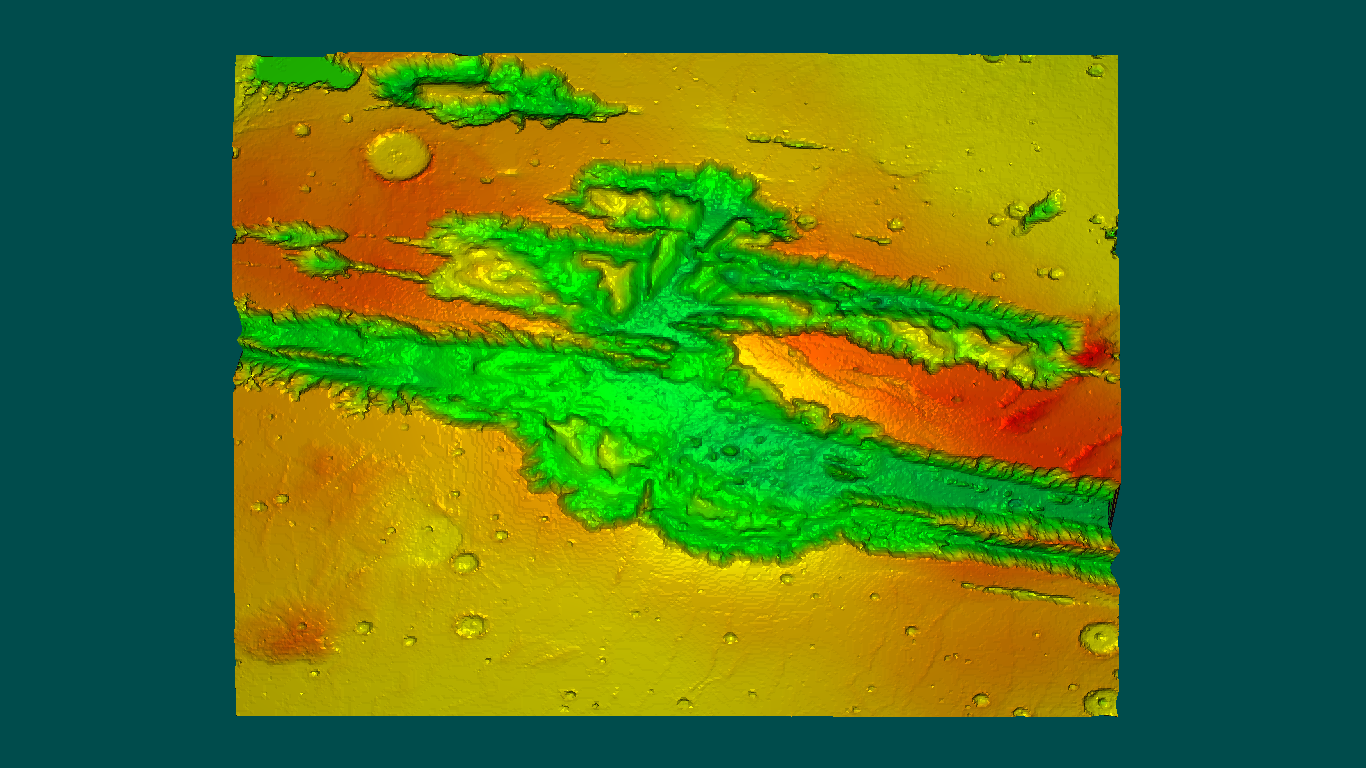
\includegraphics[width=\textwidth]{figures/myterrain.png}
	\caption[Coloreado de Valles Marineris.]{Coloreado de Valles Marineris.
	Modelo:~\cite{NASA}}
	\label{fig:myterrain}
\end{figure}

Para este problema, descrito en la sección~\ref{ref:terrain}, se ha elaborado un
vertex shader y un fragment shader. Partiendo del modelo de un terreno existen
dos posibilidades: que las alturas vengan codificadas en forma de textura o que
venga implícitamente en la posición de los vértices. En este último caso, en la
aplicación se lee el valor más alto y el valor más bajo en el eje $y$ para
realizar la coloración. 

Así, el vertex shader toma como entrada la posición y los normales de los
vértices, sacados de un modelo tridimensional.

\begin{verbatim}
    layout (location = 0) in vec3 aPos;
    layout (location = 1) in vec3 aNormal;
\end{verbatim}

Como solo se están utilizando el vertex shader y fragment shader, la salida del
vertex shader se da como entrada al fragment shader. Esta salida corresponde al
normal, que es el mismo que entra; la posición del fragmento y el color del
fragmento. Estas dos últimas variables se calculan en el vertex shader
utilizando la altura máxima y mínima del modelo, que se pasan mediante variables
\verb|uniform|.  Además, con el fin de mejorar el rendimiento, las
transformaciones de los vértices, que vienen dadas por las matrices de modelo,
vista y proyección, se calculan también en este shader. El siguiente fragmento
de código muestra las salidas del vertex shader junto con las variables
\verb|uniform| utilizadas:

\begin{verbatim}
    out vec3 vNormal;
    out vec3 vFragPos;
    out vec3 vFragColor;
    
    uniform float uMaxHeight;
    uniform float uMinHeight;
    uniform mat4 uModel;
    uniform mat4 uView;
    uniform mat4 uProjection;
\end{verbatim}

El color del fragmento se calcula realizando una interpolación entre el valor
máximo de altura(rojo), el valor tres cuartos de altura(amarillo), el valor
medio de la altura(verde) y el valor mínimo de altura(azul). El código siguiente
muestra el cálculo del color de un fragmento entre la altura máxima y los tres
cuartos:

\begin{verbatim}
    if (aPos.z > threecuarters) {
        alpha = smoothstep(uMaxHeight, threecuarters, aPos.z);	
        vFragColor = mix(RED, YELLOW, alpha);	
    }
\end{verbatim}

Asimismo, para calcular la posición del fragmento se utiliza el siguiente
código:

\begin{verbatim}		
    vFragPos = vec3(uModel * vec4(aPos, 1.0)); 
    gl_Position =  uProjection * uView * vec4(vFragPos, 1.0);
\end{verbatim}

Esto es todo lo que realiza el vertex shader, y sería suficiente para renderizar
el terreno coloreado. Sin embargo, con el fin de darle más realismo, en esta
ocasión se ha utilizado el fragment shader para dotar de iluminación a la
escena. Así, se han utilizado los normales, la posición y el color del fragmento
para elaborar un modelo de iluminación ADS~\cite{Bailey}. Esto es todo lo que
realiza el fragment shader, quedándonos lo siguiente:

\begin{verbatim}
    //Ambient
    vec3 ambient = uLight.ambient * vFragColor; 
    
    //Difuse
    vec3 norm = normalize(uNormalMatrix * vNormal);
    vec3 lightDir = normalize(uLight.position - vFragPos);
    float diff = max(dot(norm, lightDir), 0.0);
    vec3 diffuse = uLight.diffuse * (diff * vFragColor); 
    
    //Specular
    vec3 viewDir = normalize(uViewPos - vFragPos);
    vec3 reflectDir = reflect(-lightDir, norm); 
    float spec = pow(max(dot(viewDir, reflectDir), 0.0), uShininess);
    vec3 specular = uLight.specular * (spec * vFragColor);
    
    vec3 light = ambient + diffuse + specular;
    fFragColor = vec4(light, 1.0);
\end{verbatim}

El resultado final de la utilización de estos shaders se puede ver en la
figura~\ref{fig:myterrain}, para la que se ha utilizado un modelo de la NASA de
Valles Marineris, un sistema de cañones que recorre el ecuador de marte.

\subsection{Curvas de Bézier}
\label{makereference5.5.2}

Para mostrar las curvas de Bézier se han utilizado un vertex shader, un geometry
shader y un fragment shader. Además, se ha utilizado otro par de shaders para
renderizar tanto los ejes como los puntos de control de la curva. 

En este caso, todo el trabajo se realiza en el geometry shader. El vertex shader
simplemente se encarga de realizar la transformación mediante

\begin{verbatim}
    gl_Position = uProjection * uView * uModel * vec4(aPos, 1.0);
\end{verbatim}
mientras que el fragment shaders solo se encarga de darle color a la curva
mediante la instrucción

\begin{verbatim}
    fFragColor = vec4(ORANGE, 1.0);
\end{verbatim}

Así pues, veamos qué acciones realizar en el geometry shader para conseguir,
mediante los 4 vértices de control, renderizar una curva de Bézier en nuestra
aplicación. Este shader es la versión de~\citet{Bailey}. 

Recordemos de la sección~\ref{ref:GeoShader} que para el shader geométrico ha de
especificarse la primitiva de entrada y la de salida. Esto se realiza mediante
las líneas

\begin{verbatim}
    layout( lines_adjacency ) in;
    layout( line_strip, max_vertices=256 ) out;
\end{verbatim}

Utilizamos \verb|lines_adjacency| puesto que como entrada tomaremos los 4 puntos
de control (y esta es la única entrada que toma 4 puntos. Ver
tabla~\ref{tabla3.1}) y como salida \verb|line_strip| pues queremos renderizar
nuestra curva como una serie de segmentos. El nivel de detalle de nuestra curva
vendrá dado por este número de segmentos, que se especifica mediante una
variable \verb|uniform|.

\begin{verbatim}
    float dt = 1. / float(uNum);
    float t = 0.;
    for( int i  = 0; i <=uNum; i++, t+= dt){
        float omt = 1. -t;
        float omt2 = omt * omt;
        float omt3 = omt * omt2;
        float t2 = t * t;
        float t3 = t * t2;
        vec4 xyzw = omt3 * gl_PositionIn[0] +
        3. * t * omt2 * gl_PositionIn[1] +
        3. * t2 * omt * gl_PositionIn[2] +
        t3 * gl_PositionIn[3];
        gl_Position = xyzw;
        EmitVertex( );
    }
\end{verbatim}

El código anterior supone la totalidad del geometry shader. En él, mediante el
uniform \verb|uNum| indicamos la cantidad de puntos que queremos incluir de la
curva, obteniendo mayor detalle cuanto más alto es este número. El vector
\verb|xyzw| se calcula mediante la ecuación~\eqref{eq:3}. El resultado de este
shader puede verse en la Figura~\ref{fig:mybeziercurve}.

\begin{figure}
	\centering
	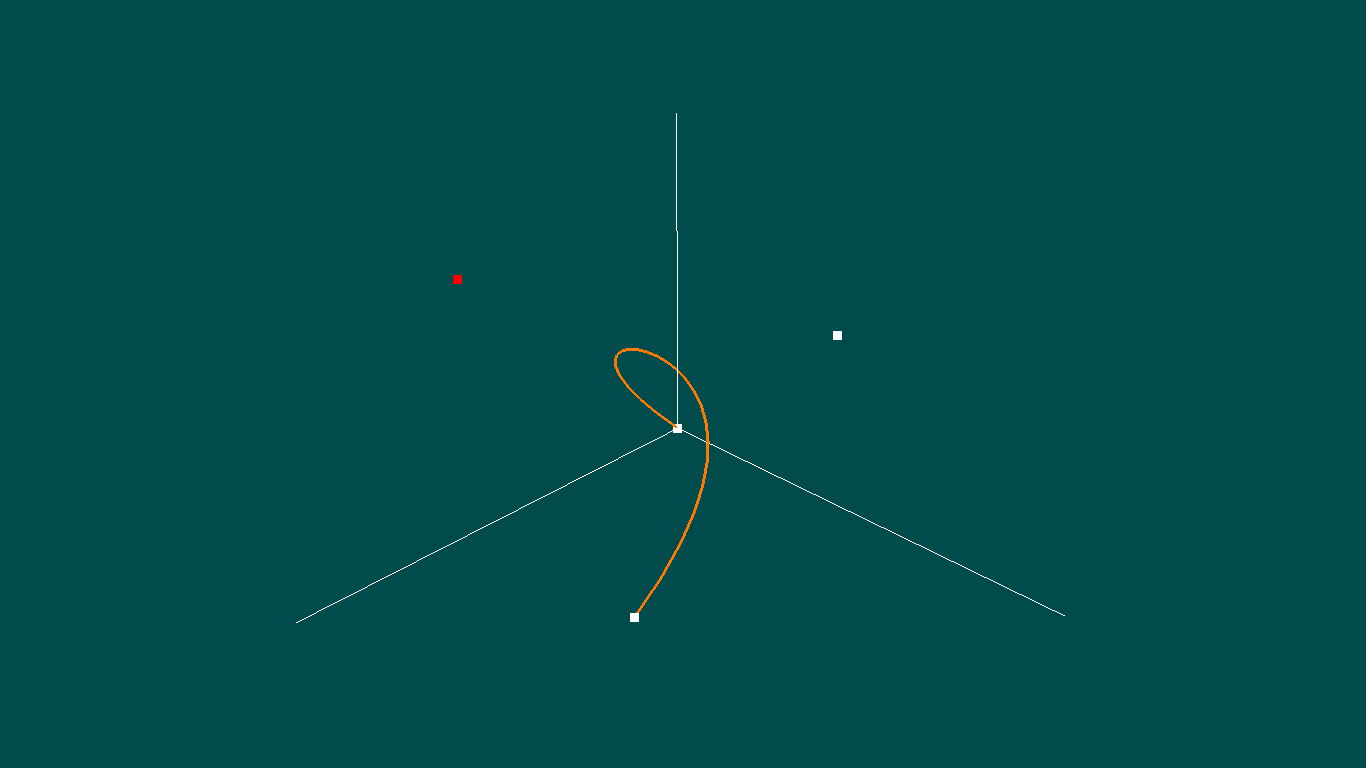
\includegraphics[width=\textwidth]{figures/mybeziercurve.png}
	\caption{Bézier Curve}
	\label{fig:mybeziercurve}
\end{figure}

\subsection{Superficies de Bézier}
\label{makereference5.5.3}

\begin{figure}
	\centering		
	\begin{subfigure}{\textwidth}
		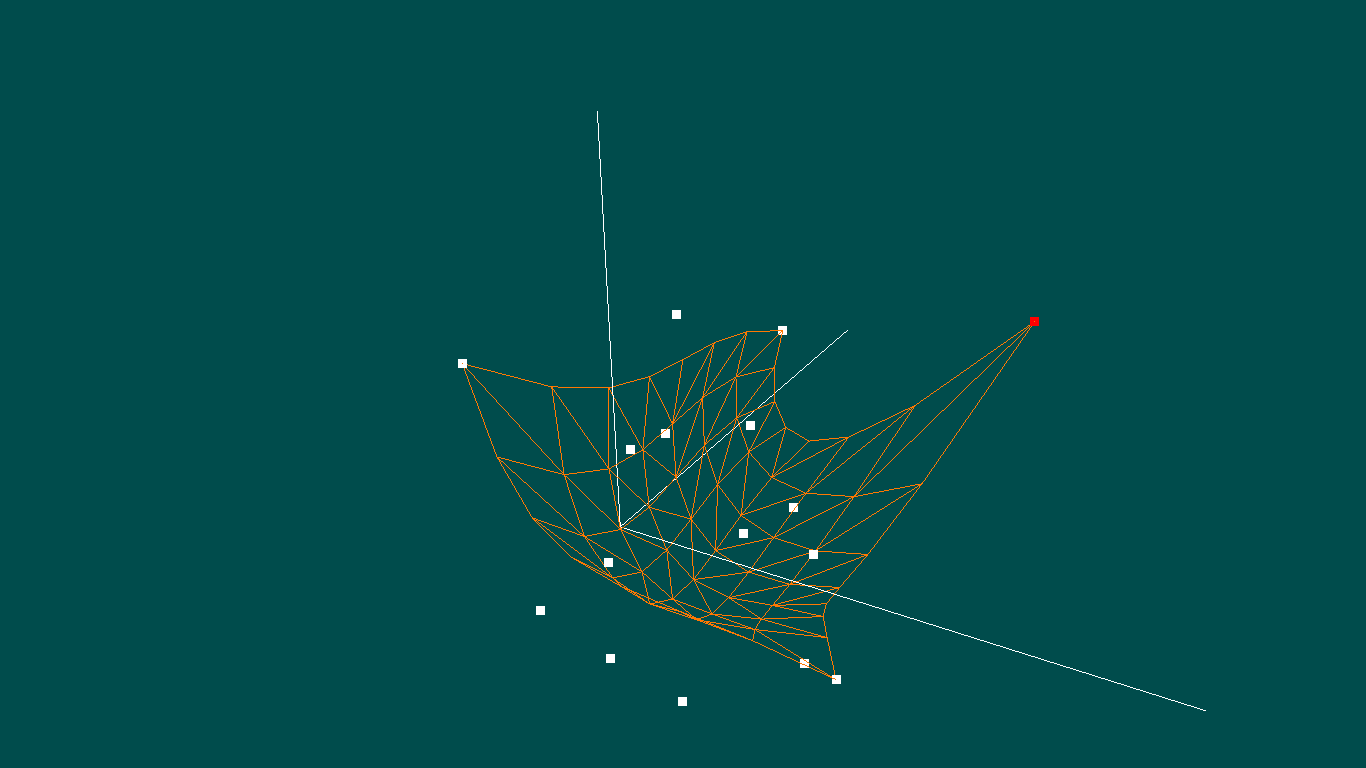
\includegraphics[width=\textwidth]{figures/mybeziersurface1.png}
	\end{subfigure}
	\newline
	\begin{subfigure}{\textwidth}
		
\includegraphics[width=\textwidth]{figures/mybeziersurface2.png}
	\end{subfigure}
	\caption{Superficie de Bézier}
	\label{fig:mybeziersurface}
\end{figure}

En este caso, en lugar de utilizar el shader geométrico como en el caso
anterior, utilizaremos los shaders de teselación. Por tanto, tendremos, al igual
que en el caso anterior, un vertex shader, un tessellation control shader, un
tessellation evaluation shader y un fragment shader, además de los mismos
shaders que en el caso anterior para renderizar los ejes y los puntos de
control. 

El vertex y fragment shader son exactamente iguales que en el caso de la curva
de Bézier, por lo que nos centraremos exclusivamente en los shaders de
teselación. El TCS ha de marcar el nivel de teselación, acorde a lo explicado en
la sección~\ref{ref:TesShaders}, y, debido a que queremos utilizar cuadriláteros
y guiándonos por la Figura~\ref{fig:quadlevels}, debemos especificar los
siguientes niveles de teselación:

\begin{verbatim}
    gl_TessLevelOuter[0] = gl_TessLevelOuter[2] = uOuter02;
    gl_TessLevelOuter[1] = gl_TessLevelOuter[3] = uOuter13;
    gl_TessLevelInner[0] = uInner0;
    gl_TessLevelInner[1] = uInner1;
\end{verbatim}

Además se pasa al TES la posición del vértice dentro del parche mediante la
instrucción:

\begin{verbatim}
    gl_out[ gl_InvocationID ].gl_Position =
        gl_in[ gl_InvocationID ].gl_Position;
\end{verbatim}

En el TES es donde realmente se realizan los cálculos necesarios para obtener la
superficie de Bézier. El siguiente código, que realiza el cálculo de la
ecuación~\eqref{eq:6} es una versión simplificada del que se puede encontrar
en~\citet{Bailey}. Este último utiliza también las propiedades de las derivadas
de las superficies de Bézier para calcular el normal con el fin de utilizar un
modelo de luz como el utilizado en~\ref{makereference5.5.1}.

\begin{verbatim}
    vec4 p00 = gl_in[0].gl_Position;
    vec4 p10 = gl_in[1].gl_Position;
    vec4 p20 = gl_in[2].gl_Position;
    vec4 p30 = gl_in[3].gl_Position;
    vec4 p01 = gl_in[4].gl_Position;
    vec4 p11 = gl_in[5].gl_Position;
    vec4 p21 = gl_in[6].gl_Position;
    vec4 p31 = gl_in[7].gl_Position;
    vec4 p02 = gl_in[8].gl_Position;
    vec4 p12 = gl_in[9].gl_Position;
    vec4 p22 = gl_in[10].gl_Position;
    vec4 p32 = gl_in[11].gl_Position;
    vec4 p03 = gl_in[12].gl_Position;
    vec4 p13 = gl_in[13].gl_Position;
    vec4 p23 = gl_in[14].gl_Position;
    vec4 p33 = gl_in[15].gl_Position;
    
    float u = gl_TessCoord.x;
    float v = gl_TessCoord.y;
    
    float bu0 = (1.-u) * (1.-u) * (1.-u);
    float bu1 = 3. * u * (1.-u) * (1.-u);
    float bu2 = 3. * u * u * (1.-u);
    float bu3 = u * u  * u;
    
    float bv0 = (1.-v) * (1.-v) * (1.-v);
    float bv1 = 3. * v * (1.-v) * (1.-v);
    float bv2 = 3. * v * v * (1.-v);
    float bv3 = v * v * v;
    
    gl_Position = 
          bu0 * ( bv0*p00 + bv1*p01 + bv2*p02 + bv3*p03 )
        + bu1 * ( bv0*p10 + bv1*p11 + bv2*p12 + bv3*p13 )
        + bu2 * ( bv0*p20 + bv1*p21 + bv2*p22 + bv3*p23 )
        + bu3 * ( bv0*p30 + bv1*p31 + bv2*p32 + bv3*p33 );

\end{verbatim}

El resultado de estos shaders se puede ver en la
Figura~\ref{fig:mybeziersurface}.

\subsection{Sólidos de revolución}
\label{makereference5.5.4}

\begin{figure}
	\centering		
	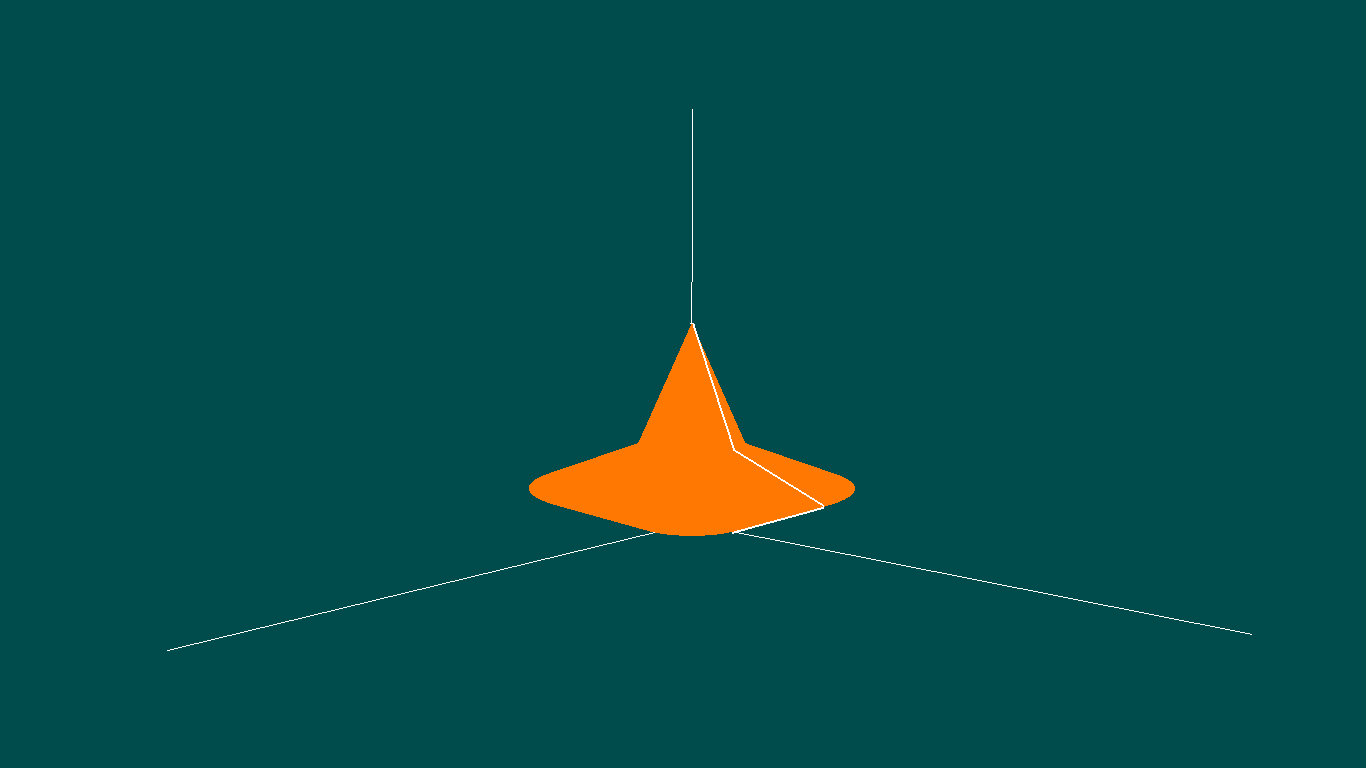
\includegraphics[width=\textwidth]{figures/myrevolution.png}
	\caption{Sólido de revolución}
	\label{fig:myrevolution}
\end{figure}

En este caso, de nuevo, tanto el vertex shader como el fragment shader son los
más simples posible, como en los casos anteriores. Todo el trabajo recae en el
geometry shader. Así, dados los vértices que forman una curva, se van generando
vértices en torno al eje $y$, tantos como indica la variable \verb|uNum|. El
resultado de revolucionar una curva en torno al eje $y$ puede verse en la
Figura~\ref{fig:myrevolution}. El código del geometry shader utilizado es el
siguiente:

\begin{verbatim}
    for( int i  = 0; i <= uNum; i++){
        float grados = 2.0*PI / uNum * i;
        
        gl_Position = gl_in[0].gl_Position;
        gl_Position.x = cos(grados)*gl_PositionIn[0].x 
		                + sin(grados)*gl_PositionIn[0].z;
        gl_Position.z = cos(grados)*gl_PositionIn[0].z 
		                - sin(grados)*gl_PositionIn[0].x;

        gl_Position = uProjection * uView * uModel * gl_Position;
        EmitVertex( );
        
        gl_Position = gl_PositionIn[1];
        gl_Position.x = cos(grados)*gl_PositionIn[1].x 
		                + sin(grados)*gl_PositionIn[1].z;
        gl_Position.z = cos(grados)*gl_PositionIn[1].z 
		                - sin(grados)*gl_PositionIn[1].x;

        gl_Position = uProjection * uView * uModel * gl_Position;
        EmitVertex( );
    }
\end{verbatim}

\subsection{Nube de puntos}
\label{makereference5.5.5}

\begin{figure}[h]
	\centering	
	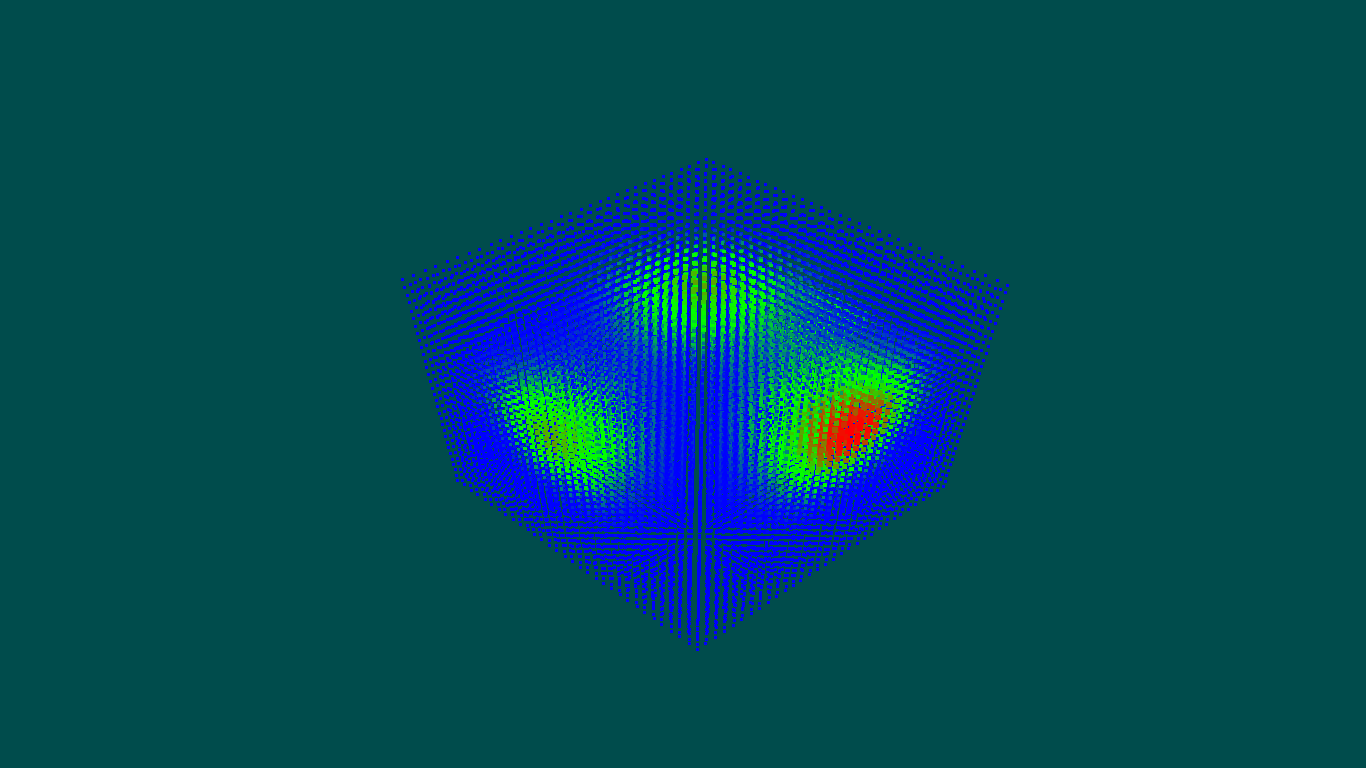
\includegraphics[width=\textwidth]{figures/mycloud.png}
	\caption{Nube de puntos}
	\label{fig:mycloud}
\end{figure}

Para realizar esta visualización se han utilizado únicamente un vertex shader y
un fragment shader. Como entradas, el vertex shader utiliza tanto la posición
del vértice en la nube de puntos como el escalar que representa la información
que queremos visualizar. 

En el vertex shader, además de definir la posición mediante las transformaciones
necesarias, utilizamos la siguiente instrucción

\begin{verbatim}
    gl_PointSize = 2 + pow((smoothstep(0.0, uMaxData, aScalar) + 1), 2);
\end{verbatim}

para definir el tamaño del punto acorde al escalar. Así, los puntos que se
correspondan con escalares más altos tendrán un tamaño mayor. El valor escalar
\verb|aScalar| es pasado también al fragment shader para realizar una coloración
del punto acorde a este valor. 

\begin{figure}[hb]
	\centering	
	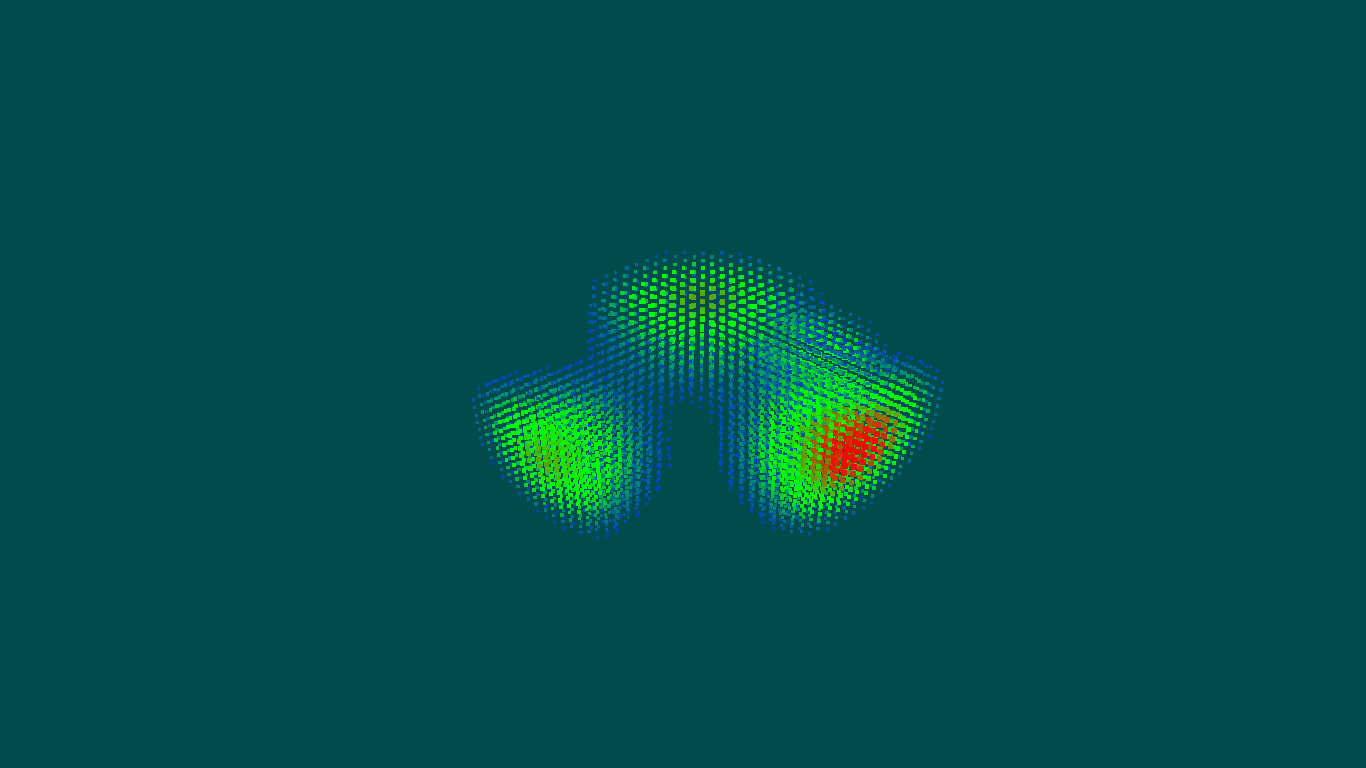
\includegraphics[width=\textwidth]{figures/mycloud2.png}
	\caption{Nube de puntos con valores descartados}
	\label{fig:mycloud2}
\end{figure}

Además, en el fragment shader se ha declarado la variable \verb|uniform uMax|
que se utiliza para descartar los puntos que tengan valores escalares menores
que él. Así, podemos visualizar de una manera  más efectiva datos por encima de
cierto límite. Este comportamiento puede verse en la Figura~\ref{fig:mycloud2}.
El código para este shader se incluye a continuación.

\begin{verbatim}
    if(vScalar < uMax) discard;	
    float alpha;
    float middle = uMaxData / 2;
    if(vScalar >= middle){
        alpha = smoothstep(middle, uMaxData, vScalar);
        fFragColor = vec4(mix(GREEN, RED, alpha), 1.0f);
    }
    else{
        alpha = smoothstep(0.0, middle, vScalar);
        fFragColor = vec4(mix(BLUE, GREEN, alpha), 1.0f);
    }
\end{verbatim}

\subsection{Negativo de una imagen}
\label{makereference5.5.6}

\begin{figure}[h]
	\centering	
	\begin{subfigure}{0.45\textwidth}
		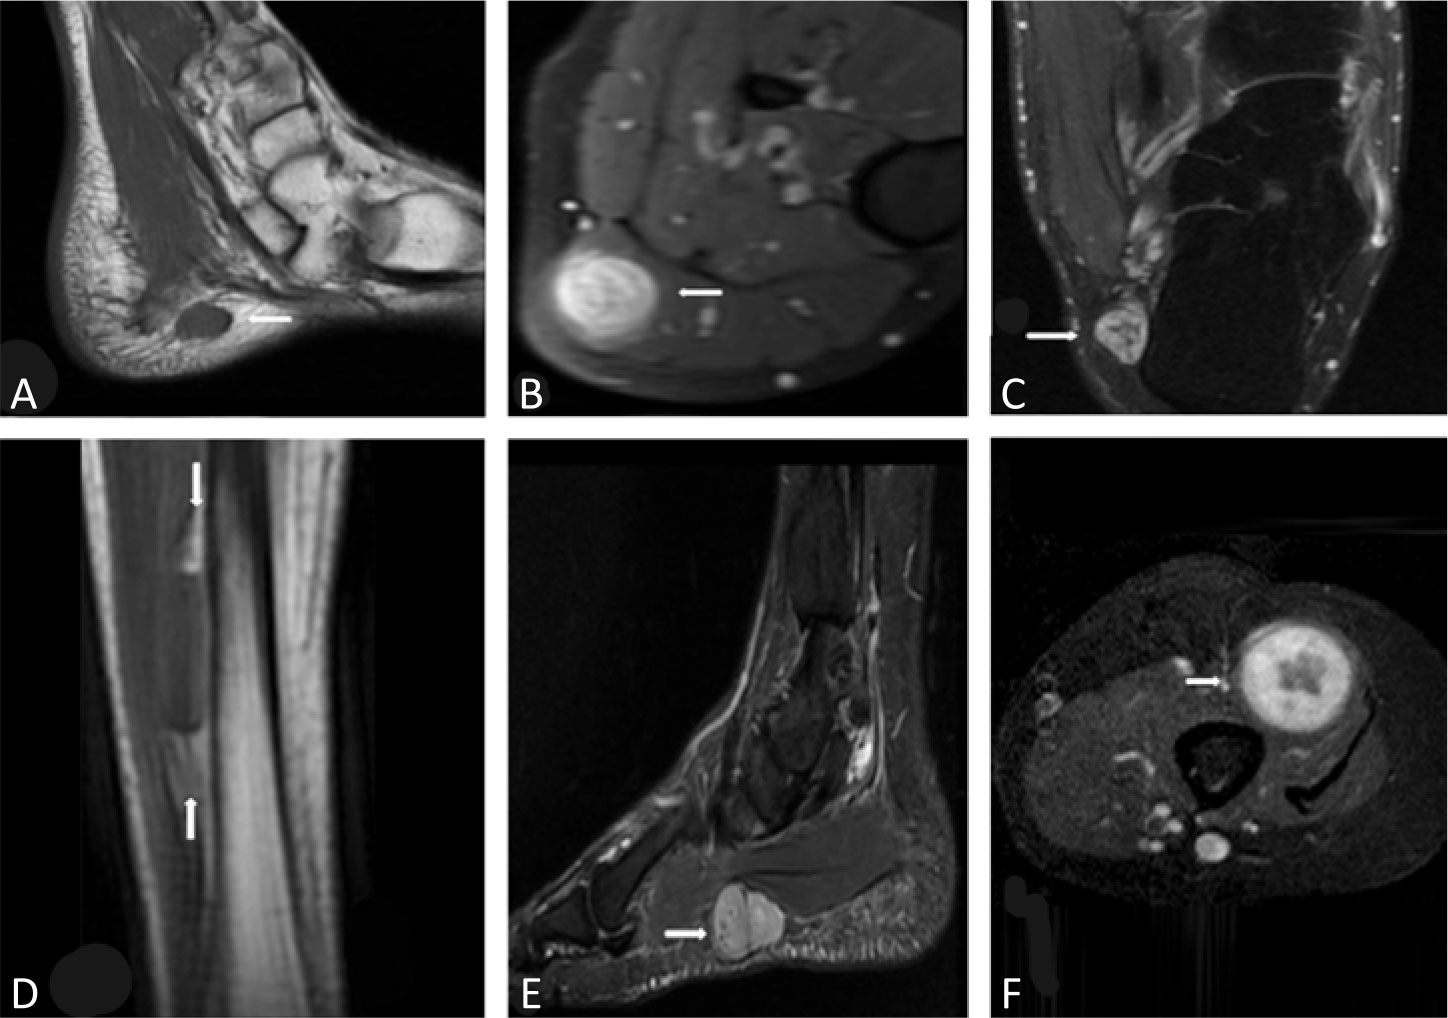
\includegraphics[height=8cm,width=\textwidth]{figures/mynegative00.jpg}
		\caption{Imagen original}
	\end{subfigure}
	\hfill
	\begin{subfigure}{0.45\textwidth}
		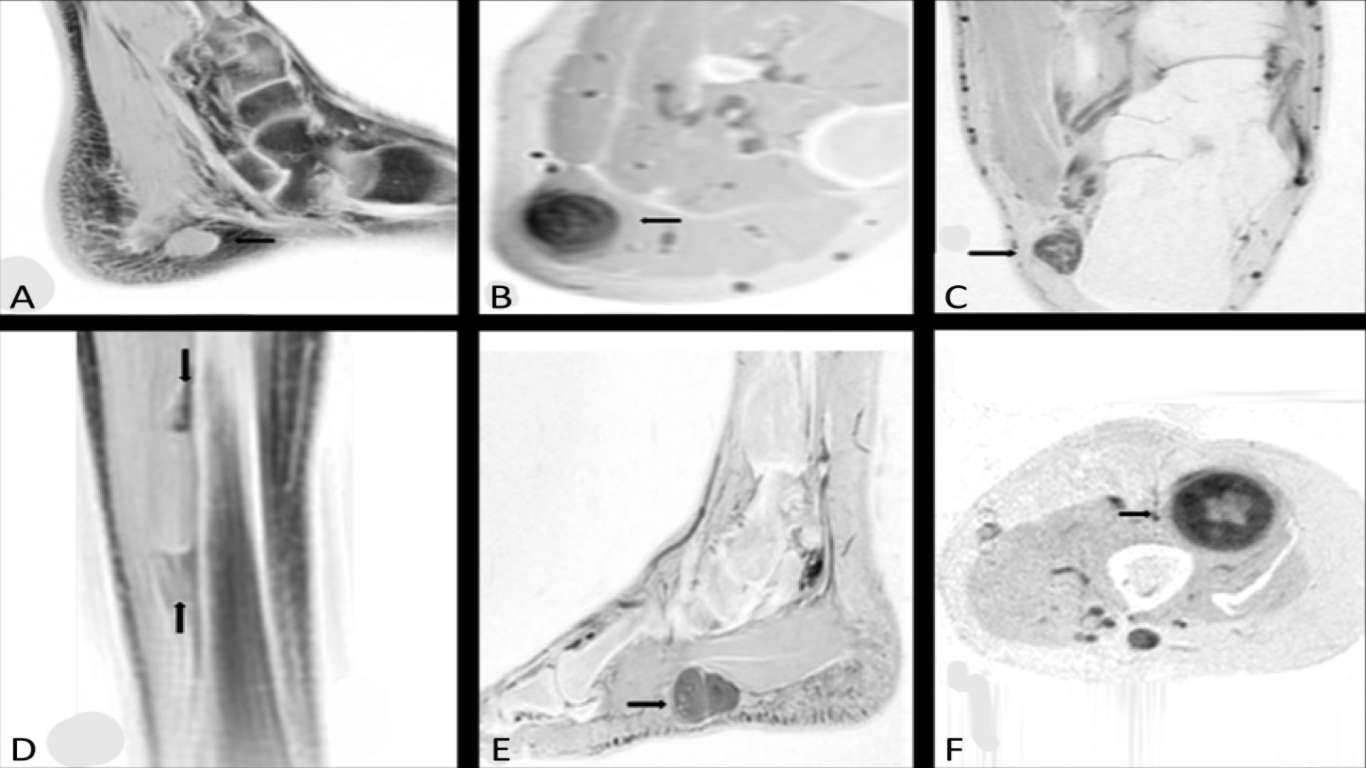
\includegraphics[height=8cm,width=\textwidth]{figures/mynegative01.png}
		\caption{Negativo}
	\end{subfigure}
	\caption[Negativo de una imagen.]{Negativo de una imagen.
	Fuente:~\cite{negativeimage}}
	\label{fig:mynegative}
\end{figure}

En este caso, al tratarse de una imagen, los únicos elementos que necesitamos
son cuatro vértices cuya posición se corresponda con cada una de las esquinas de
la imagen y la textura para la imagen. Así pues, el vertex shader toma como
entrada la posición de estos cuatro vértices junto a las coordenadas que le
corresponden en la textura. Estas coordenadas de textura se definen en el
intervalo $(0,1)\times(0,1)$, siendo el punto $(0,0)$ la esquina inferior
izquierda de la textura y el punto $(1,1)$ la esquina superior derecha. Con
estos datos, el vertex shader escribe la posición de los cuatro vértices y pasa
las coordenadas de textura al fragment shader, que es el que las utilizará. 

El fragment shader, por su parte, obtiene el color original de los fragmentos
con la instrucción

\begin{verbatim}
    vec3 irgb = texture( texture1, vTexCoords ).rgb;
\end{verbatim}

para posteriormente computar el color negativo y escribirlo como salida para el
pixel. Esta tarea se realiza con las siguientes instrucciones:

\begin{verbatim}
    vec3 neg = vec3(1.,1.,1.) - irgb;
    fFragColor = vec4( mix( irgb, neg, uT ), 1. );
\end{verbatim}

Una muestra del funcionamiento de este shader se puede encontrar en la
Figura~\ref{fig:mynegative}.

% \subsection{Detección de bordes}
% \label{makereference5.5.7}
% 
% \begin{figure}
% 	\centering	
% 	\includegraphics[width=\textwidth]{figures/myborder.png}
% 	\caption{Detección de bordes}
% 	\label{fig:myborder}
% \end{figure}

\subsection{Line Integral Convolution}
\label{makereference5.5.8}

El caso del Line Integral Convolution presenta un problema a la hora de realizar
mediante un shader los cálculos necesarios. Esto se debe a que, como hemos visto
anteriormente, necesitamos, para calcular la línea de flujo, los valores del
campo vectorial de los demás vértices, algo que no podemos, a priori, obtener en
un shader. La solución para este problema consiste en codificar en forma de
textura la información del campo vectorial asociado al problema. 

\begin{figure}[b]
	\centering	
	\begin{subfigure}{0.7\textwidth}
			\includegraphics[width=\textwidth]{figures/lictexture2.png}	
	\end{subfigure}
	\begin{subfigure}{0.28\textwidth}
			\includegraphics[width=\textwidth]{figures/lictexture.png}	
	\end{subfigure}
	\caption[LIC - Información del campo vectorial codificado en una
	textura.]{LIC - Información del campo vectorial codificado en una textura.
	Fuente:~\cite{Bailey}}
	\label{fig:lictexture}
\end{figure}

Para ello, como se explica en~\citet{Bailey} y como se puede observar en la
Figura~\ref{fig:lictexture}, se asocia a cada punto del campo un color
dependiendo de los valores de las componentes vectoriales de dicho punto. A
mayor valor de la coordenada $x$ se le asocia un valor más alto del color rojo
siguiendo el convenio RGB. Similarmente, a mayor valor de la coordenada $y$ se
le asocia un valor mayor del color verde. 

\begin{figure}
	\centering	
	\begin{subfigure}{0.45\textwidth}
		\includegraphics[height=\textwidth,width=\textwidth]{figures/mylic.png}
		\caption{Lic para el flujo vectorial de debajo.}
		\label{fig:mylic1}
	\end{subfigure}
	\hfill
	\begin{subfigure}{0.45\textwidth}
		\includegraphics[height=\textwidth,width=\textwidth]{figures/mylic2.png}
		\caption{Lic para el flujo vectorial de debajo.}
		\label{fig:mylic2}
	\end{subfigure}
	\newline 
	\par\bigskip\par\bigskip
	\begin{subfigure}{0.45\textwidth}
		\includegraphics[height=\textwidth,width=\textwidth]{figures/mylic3.jpg}
		\caption{Flujo vectorial codificado en textura.}
		\label{fig:mylic3}
	\end{subfigure}
	\hfill
	\begin{subfigure}{0.45\textwidth}
		\includegraphics[height=\textwidth,width=\textwidth]{figures/mylic4.png}
		\caption{Flujo vectorial codificado en textura.}
		\label{fig:mylic4}
	\end{subfigure}
	\caption{Line Integral Convolution.}
	\label{fig:mylic}
\end{figure}

Las texturas con estos valores así calculados tienen un aspecto similar al de las
Figuras~\ref{fig:mylic3} y~\ref{fig:mylic4}, dependiendo del flujo vectorial
subyacente.

Para esta técnica necesitaremos solo un vertex shader y un fragment shader. El
vertex shader toma de nuevo la posición de los vértices, que en este caso se
trata de una malla de $256\times 256$ vértices y las coordenadas de textura de
cada uno de ellos. Este shader simplemente pasa las coordenadas de textura al
fragment shader y escribe la posición del vértice. 

El fragment shader toma las coordenadas de textura procedentes del vertex shader
y realiza las operaciones explicadas en la sección~\ref{ref:lic}. Primero
realiza, para cada vértice, el cómputo de la línea de flujo mediante el método
de Runge-Kutta de orden 4. Para este método se define el tamaño del paso
mediante la variable \verb|stp| y la longitud de la línea de flujo que queremos
calcular mediante la variable \verb|uniform uLength|.

\begin{verbatim}
    vec3 color = texture( texture1, vTexCoords ).rgb;
    vec2 st = vTexCoords;
    float stp = 0.00281;

    // Cálculo de la línea de flujo en dirección positiva
    for( int i = 0; i < uLength; i++ )
    {
        vec2 k1 = texture( texture2, st ).xy;
        vec2 k2 = texture( texture2, st + k1*stp/2 ).xy;
        vec2 k3 = texture( texture2, st + k2*stp/2 ).xy;
        vec2 k4 = texture( texture2, st + k3*stp).xy;
        vec2 ks = k1 + 2*k2 + 2*k3 + k4;
        st += stp/6*ks;
        st = clamp( st, 0., 1. );
        color += vec3( texture( texture1, st ) );
    }

    // Cálculo de la línea de flujo en dirección negativa
    st = vTexCoords;
    for( int i = 0; i < uLength; i++ )
    {
        vec2 k1 = texture( texture2, st ).xy;
        vec2 k2 = texture( texture2, st - k1 * stp / 2 ).xy;
        vec2 k3 = texture( texture2, st - k2 * stp / 2 ).xy;
        vec2 k4 = texture( texture2, st - stp*k3).xy;
        vec2 ks = k1 + 2*k2 + 2*k3 + k4;
        st -= stp/6*ks;
        st = clamp( st, 0., 1. );
        color += vec3( texture( texture1, st ) );
    }
    color /= float(2*uLength + 1); 
\end{verbatim}

En este shader se ha omitido el cálculo de los pesos, tomando como valor para
ellos $1$ en todos los casos y dividiendo por el número de puntos en la línea
de flujo. Con todo esto en cuenta, el resultado final se puede observar en la
Figura~\ref{fig:mylic}.

\subsection{Uso de la aplicación}
\label{subsection:uso}

Una vez visto el diseño de la aplicación y los shaders utilizados, se presenta
el modo de utilización de la aplicación. Una vez conseguido el ejecutable, para
esta explicación llamado \verb|tfg| se debe ejecutar con alguno de los modos de
visualización explicados anteriormente. Cada uno de estos modos permite unas
opciones de visualización diferentes, que se explican a continuación.

Además, todos los modos comparten el movimiento de la cámara, que es el
siguiente:

\begin{itemize}
		\item \verb|Esc| - Salir.
		\item \verb|w| - Mover la cámara hacia delante.
		\item \verb|s| - Mover la cámara hacia atrás.
		\item \verb|d| - Mover la cámara hacia la derecha.
		\item \verb|a| - Mover la cámara hacia la izquierda.
\end{itemize}

Junto con el movimiento del ratón, que cambia el objetivo al que apunta la
cámara, y la ruleta del ratón, que permite hacer y deshacer zoom.

\subsubsection{Visualización de Terrenos}

\verb|$ ./tfg terrain|

Opciones: No tiene opciones especiales.

\subsubsection{Curva de Bézier}

\verb|$ ./tfg bezier|

La aplicación permite aumentar y disminuir el número de vértices de la curva,
así como mover los puntos de control.
Opciones:

\begin{itemize}
		\item \verb|\textvisiblespace| - Seleccionar siguiente vértice.
		\item \verb|\uparrow| - Aumentar número de segmentos.
		\item \verb|\downarrow| - Disminuir número de segmentos.
		\item \verb|x| - Mover el vértice seleccionado en la dirección $+x$.
		\item \verb|y| - Mover el vértice seleccionado en la dirección $+y$.
		\item \verb|z| - Mover el vértice seleccionado en la dirección $+z$.
		\item \verb|Shift + x| - Mover el vértice seleccionado en la dirección $-x$.
		\item \verb|Shift + y| - Mover el vértice seleccionado en la dirección $-y$.
		\item \verb|Shift + z| - Mover el vértice seleccionado en la dirección $-z$.
\end{itemize}

\subsubsection{Superficie de Bézier}

\verb|$ ./tfg bsurface|

La aplicación permite aumentar y disminuir el grado de teselación de la
superficie, así como mover los puntos de control.  
Opciones:

\begin{itemize}
		\item \verb|\textvisiblespace| - Seleccionar siguiente vértice.
		\item \verb|\uparrow| - Aumentar grado de teselación.
		\item \verb|\downarrow| - Disminuir grado de teselación.
		\item \verb|t| - Activar el modo wireframe
		\item \verb|u| - Desactivar el modo wireframe
		\item \verb|x| - Mover el vértice seleccionado en la dirección $+x$.
		\item \verb|y| - Mover el vértice seleccionado en la dirección $+y$.
		\item \verb|z| - Mover el vértice seleccionado en la dirección $+z$.
		\item \verb|Shift + x| - Mover el vértice seleccionado en la dirección $-x$.
		\item \verb|Shift + y| - Mover el vértice seleccionado en la dirección $-y$.
		\item \verb|Shift + z| - Mover el vértice seleccionado en la dirección $-z$.
\end{itemize}

\subsubsection{Nube de puntos}

\verb|$ ./tfg cloud|

Opciones:

\begin{itemize}
		\item \verb|\uparrow| - Aumentar límite para el escalar.
		\item \verb|\downarrow| - Disminuir límite para el escalar.
\end{itemize}

\subsubsection{Negativo}

\verb|$ ./tfg negative|

Opciones: No tiene opciones especiales

\subsubsection{Sólido de revolución}

\verb|$ ./tfg revolution|

Opciones:

\begin{itemize}
		\item \verb|\uparrow| - Aumentar número de vértices de revolución.
		\item \verb|\downarrow| - Disminuir número de vértices de revolución.
		\item \verb|t| - Activar el modo wireframe
		\item \verb|u| - Desactivar el modo wireframe
\end{itemize}

\subsubsection{Line Integral Convolution}

\verb|$ ./tfg lic|

Opciones:

\begin{itemize}
		\item \verb|\uparrow| - Aumentar longitud de la línea de flujo.
		\item \verb|\downarrow| - Disminuir longitud de la línea de flujo.
\end{itemize}

\cleardoublepage

\chapter{Conclusiones y Trabajo Futuro}
\label{makereference6}

\subsection{Conclusiones}

Con este trabajo he conseguido entender cómo funcionan la informática gráfica y
cómo utilizarla para visualización científica. He podido observar como es un
campo relativamente nuevo pero creciendo a una gran velocidad y ganando cada vez
más importancia.

He podido observar la enorme utilidad que puede llegar a tener la visualización
y la gran ayuda que puede suponer para los equipos que trabajan con grandes
volúmenes de datos. También he podido ser consciente como equipos científicos
enormemente importantes utilizan estas técnicas para realizar descubrimientos
pioneros, como es el caso del EHT~\cite{EHT} con la obtención de la primera imagen
de un agujero negro~\cite{1435174}.

\subsection{Posible Trabajo Futuro}
Como trabajo futuro se plantean varios puntos:

\begin{itemize}

		\item Seguir aprendiendo sobre el tema y alcanzar un mayor
				conocimiento que permita entender las últimas tendencias y
				descubrimientos en este área.

		\item Conocer más técnicas de visualización e incorporarlas a la
				aplicación.

		\item Mejorar la aplicación con la introducción de cuaterniones.

		\item Mejorar la aplicación con la posibilidad de realizar los tipos
				de visualización a partir de modelos y ficheros especificados
				por el usuario.

		\item Profundizar en la visualización de fluidos y en los nuevos
				métodos tridimensionales.

\end{itemize}


\bibdata{references}
\bibliography{references}
\addcontentsline{toc}{chapter}{Referencias}

\appendix
% +--------------------------------------------------------------------+
% | Appendix A Page (Optional)                                         |
% +--------------------------------------------------------------------+

\cleardoublepage

\chapter{Title for This Appendix}
\label{Appendix:Key1}


% +--------------------------------------------------------------------+
% | Enter text for your Appendix page in the space below this box.     |
% |                                                                    |
% +--------------------------------------------------------------------+


\end{document}
